% Options for packages loaded elsewhere
\PassOptionsToPackage{unicode}{hyperref}
\PassOptionsToPackage{hyphens}{url}
\PassOptionsToPackage{dvipsnames,svgnames,x11names}{xcolor}
%
\documentclass[
  11pt,
]{article}
\usepackage{amsmath,amssymb}
\usepackage{setspace}
\usepackage{iftex}
\ifPDFTeX
  \usepackage[T1]{fontenc}
  \usepackage[utf8]{inputenc}
  \usepackage{textcomp} % provide euro and other symbols
\else % if luatex or xetex
  \usepackage{unicode-math} % this also loads fontspec
  \defaultfontfeatures{Scale=MatchLowercase}
  \defaultfontfeatures[\rmfamily]{Ligatures=TeX,Scale=1}
\fi
\usepackage{lmodern}
\ifPDFTeX\else
  % xetex/luatex font selection
\fi
% Use upquote if available, for straight quotes in verbatim environments
\IfFileExists{upquote.sty}{\usepackage{upquote}}{}
\IfFileExists{microtype.sty}{% use microtype if available
  \usepackage[]{microtype}
  \UseMicrotypeSet[protrusion]{basicmath} % disable protrusion for tt fonts
}{}
\makeatletter
\@ifundefined{KOMAClassName}{% if non-KOMA class
  \IfFileExists{parskip.sty}{%
    \usepackage{parskip}
  }{% else
    \setlength{\parindent}{0pt}
    \setlength{\parskip}{6pt plus 2pt minus 1pt}}
}{% if KOMA class
  \KOMAoptions{parskip=half}}
\makeatother
\usepackage{xcolor}
\usepackage[margin=2.5cm]{geometry}
\usepackage{longtable,booktabs,array}
\usepackage{calc} % for calculating minipage widths
% Correct order of tables after \paragraph or \subparagraph
\usepackage{etoolbox}
\makeatletter
\patchcmd\longtable{\par}{\if@noskipsec\mbox{}\fi\par}{}{}
\makeatother
% Allow footnotes in longtable head/foot
\IfFileExists{footnotehyper.sty}{\usepackage{footnotehyper}}{\usepackage{footnote}}
\makesavenoteenv{longtable}
\usepackage{graphicx}
\makeatletter
\def\maxwidth{\ifdim\Gin@nat@width>\linewidth\linewidth\else\Gin@nat@width\fi}
\def\maxheight{\ifdim\Gin@nat@height>\textheight\textheight\else\Gin@nat@height\fi}
\makeatother
% Scale images if necessary, so that they will not overflow the page
% margins by default, and it is still possible to overwrite the defaults
% using explicit options in \includegraphics[width, height, ...]{}
\setkeys{Gin}{width=\maxwidth,height=\maxheight,keepaspectratio}
% Set default figure placement to htbp
\makeatletter
\def\fps@figure{htbp}
\makeatother
\setlength{\emergencystretch}{3em} % prevent overfull lines
\providecommand{\tightlist}{%
  \setlength{\itemsep}{0pt}\setlength{\parskip}{0pt}}
\setcounter{secnumdepth}{-\maxdimen} % remove section numbering
\usepackage{amsmath}
\usepackage{float}
\usepackage{xurl}
\usepackage{ragged2e}
\let\origfigure\figure
\let\endorigfigure\endfigure
\renewenvironment{figure}[1][2] {\origfigure[H]\centering} {\endorigfigure}
\usepackage{caption}
\captionsetup{font=small,labelformat=empty,justification=justified,singlelinecheck=false}
\setlength{\emergencystretch}{3em}
\setlength{\parindent}{0pt}
\setlength{\parskip}{4pt}
\usepackage{titlesec}
\titlespacing*{\section}{0pt}{12pt}{6pt}
\titlespacing*{\subsection}{0pt}{9pt}{4pt}
\usepackage{needspace}
\ifLuaTeX
  \usepackage{selnolig}  % disable illegal ligatures
\fi
\IfFileExists{bookmark.sty}{\usepackage{bookmark}}{\usepackage{hyperref}}
\IfFileExists{xurl.sty}{\usepackage{xurl}}{} % add URL line breaks if available
\urlstyle{same}
\hypersetup{
  pdftitle={Wave Aware Risk Controlled Link Selection for Hybrid LoRa and LEO Satellite Ocean Monitoring IoT},
  pdfauthor={G. Arul Dalton1,* and S. V. J. Mani2; 1Department of Computer Science and Engineering, Saveetha Engineering College,; Chennai, Tamil Nadu, India. E-mail: aruldalton@saveetha.ac.in; 2Department of Computer Science Engineering and Cyber Security,; Saveetha Engineering College, Chennai, Tamil Nadu, India.; E-mail: manisvj@saveetha.ac.in; *Corresponding author: G. Arul Dalton, aruldalton@saveetha.ac.in; ORCID: G. Arul Dalton 0000-0002-5981-7176},
  colorlinks=true,
  linkcolor={black},
  filecolor={Maroon},
  citecolor={Blue},
  urlcolor={blue},
  pdfcreator={LaTeX via pandoc}}

\title{Wave Aware Risk Controlled Link Selection for Hybrid LoRa and LEO
Satellite Ocean Monitoring IoT}
\author{G. Arul Dalton\textsuperscript{1,*} and S. V. J.
Mani\textsuperscript{2} \and \textsuperscript{1}Department of Computer
Science and Engineering, Saveetha Engineering College, \and Chennai,
Tamil Nadu, India. E-mail:
aruldalton@saveetha.ac.in \and \textsuperscript{2}Department of Computer
Science Engineering and Cyber Security, \and Saveetha Engineering
College, Chennai, Tamil Nadu, India. \and E-mail:
manisvj@saveetha.ac.in \and \textsuperscript{*}Corresponding author: G.
Arul Dalton, aruldalton@saveetha.ac.in \and ORCID: G. Arul Dalton
0000-0002-5981-7176}
\date{}

\begin{document}
\maketitle

\setstretch{1.15}
\hypertarget{abstract}{%
\section*{Abstract}\label{abstract}}
\addcontentsline{toc}{section}{Abstract}

Ocean monitoring buoys must decide, packet by packet, whether to
transmit over a cheap but fragile LoRa link to a shore gateway, over an
expensive direct-to-satellite LR-FHSS link during a low Earth orbit
pass, or to buffer the reading. Learned link-adaptation schemes optimise
average reward but cannot state how often their decisions will fail.
This paper introduces WARDEN, a wave aware decision engine with a
certified failure rate. A closed-form physics prior integrates the
two-ray sea channel over the heave measured by the buoy's inertial
sensor; an attention network with sea-state-conditioned cross attention
and a spreading-factor-monotone head learns the residual. A Mondrian
Learn-then-Test calibration certifies, per sea state, that the
attempt-failure probability stays below a target α, and adaptive
conformal updates organised in urgency-aware cells keep this guarantee
under distribution shift while rescuing readings about to expire. In a
60-day, 20-buoy physics-based test bed, WARDEN held the failure rate at
5\% in every sea state, under severe storms and after a site change,
delivered 84.5--90.0\% of all readings, matching or exceeding an
adaptive-data-rate rule that failed 10--20\% of its attempts, and used
4.2--4.6 times less energy per reading. The guarantee survived a
deliberately misspecified physics model.

\textbf{Keywords:} Maritime Internet of Things; LoRa and LR-FHSS;
Direct-to-satellite IoT; Conformal risk control; Physics-informed
learning; Attention networks

\hypertarget{introduction}{%
\section{1 Introduction}\label{introduction}}

Buoys, gliders and moored platforms produce the temperature, wave and
water-quality records on which ocean forecasting and environmental
protection depend, yet the radio link that carries these records is the
weakest part of most deployments {[}1--4{]}. Cellular coverage fades a
few kilometres offshore, and practical maritime IoT therefore relies on
low-power wide-area links such as LoRaWAN towards gateways on shore or
on offshore platforms {[}5{]}, complemented by satellite connectivity
where no terrestrial infrastructure exists {[}3, 6, 7{]}. Field
campaigns show that offshore LoRa links are strongly modulated by the
sea itself: received power depends on antenna height above the
instantaneous surface, wave crests intermittently screen low antennas,
and humidity-driven refraction varies through the day {[}5, 8{]}.
Channel studies for ship-to-ship, UAV-to-ship and over-the-horizon links
confirm that maritime propagation is non-stationary and weather
dependent {[}9--12{]}, and hybrid satellite, aerial and terrestrial
architectures have been proposed to bridge coverage gaps {[}3, 13,
14{]}.

Direct-to-satellite (DtS) IoT has recently become a realistic second
path for buoys. LR-FHSS extends the LoRa ecosystem towards LEO gateways
{[}15, 16{]}, and analyses of Doppler effects, uplink scheduling and
Arctic buoy trials map its limits {[}17--19{]}. The satellite path,
however, is available only during passes, needs high transmit power and
long frames, and is itself degraded at low elevation {[}16--18{]}. A
monitoring buoy therefore faces a recurring decision with a real energy
price: use LoRa with a small spreading factor (SF), raise the SF, wait
for a pass, or defer the reading.

Learning-based link adaptation is the current answer to this decision.
Attention and Transformer models predict wireless channels accurately
{[}20--22{]}, machine-learning link-failure predictors have been
reported for LoRa networks {[}23, 24{]}, and deep-learning and
reinforcement-learning variants of LoRaWAN adaptive data rate (ADR) now
tune the SF from observed link metrics {[}25--27{]}, including an
LSTM-assisted deep reinforcement learning controller designed
specifically for two-ray maritime channels {[}25{]}. Inertial sensors
have even been shown to predict received power on water-surface nodes
{[}28{]}. All of these schemes optimise an average reward or an accuracy
metric. None of them states how often its decisions will fail, and none
keeps that number under control when a storm or a new site changes the
channel. Conformal prediction supplies exactly such statements for AI
models in communication systems {[}29--31{]}, and risk-controlling
extensions certify general losses {[}32--34{]} or track a target error
rate under drift {[}35{]}. These guarantees have not yet been connected
with sea-state physics or with the hybrid LoRa and satellite choice
faced by an ocean buoy.

This paper closes that gap with WARDEN (Wave-Aware Risk-controlled
DEcision eNgine). Its contributions are:

\begin{enumerate}
\def\labelenumi{\arabic{enumi}.}
\tightlist
\item
  \textbf{Certified hybrid link selection for ocean IoT.} Per-packet
  selection among LoRa SF7--SF12, an LR-FHSS satellite frame and
  buffering is cast as energy-minimising \emph{selective prediction}
  under an explicit attempt-failure constraint, and solved with a
  finite-sample guarantee that holds separately in calm, moderate and
  rough seas. To the best of our knowledge this is the first
  link-selection scheme for maritime IoT with a per-sea-state
  reliability certificate.
\item
  \textbf{Physics-informed wave prior with attention residual learning
  (WARDEN-PI).} A closed-form prior integrates the two-ray sea channel
  over the IMU-measured heave distribution by Gauss--Hermite quadrature
  and adds blockage, tide and satellite geometry. WARDEN-Net, a
  sea-state-conditioned cross-attention network with an SF-monotone
  head, learns only the residual that physics cannot explain (shadowing,
  ducting, interference).
\item
  \textbf{Urgency-aware Mondrian certification (WARDEN-U).} Risk budgets
  are allocated jointly by sea state and by data urgency: epochs in
  which a buffered reading is about to expire form their own
  certification cell with their own target. This lifts the reading
  delivery ratio to the level of ADR while keeping the certified failure
  rate of ordinary traffic.
\item
  \textbf{Certification that survives a wrong physics model.} A
  Learn-then-Test calibration that needs no monotone loss is combined
  with adaptive conformal updates driven by the gateway's receipt
  bitmap. The guarantee is shown to hold under severe storms, under a
  site and hardware shift, and when the physics prior is deliberately
  misspecified.
\item
  \textbf{A reproducible sandbox test bed} with tides, wave heave and
  tilt, blockage, ducting, LEO passes and LR-FHSS, two
  out-of-distribution deployments, physics-prior misspecification, full
  ablations and open code.
\end{enumerate}

Section 2 reviews related work. Section 3 defines the system model, the
problem statements and the research gap. Section 4 presents the
algorithm. Sections 5 to 7 report the experimental setup, results and
ablations, and Sections 8 and 9 discuss limitations and conclude.

\hypertarget{related-work}{%
\section{2 Related work}\label{related-work}}

\textbf{Maritime IoT communication.} Surveys of the maritime IoT
describe a layered architecture in which coastal base stations,
satellites and, increasingly, aerial relays share the task of serving
vessels and buoys {[}1--3{]}. Xia et al.~{[}1{]} identify the radio
spectrum and the air interface as the main obstacles to machine-type
maritime communication. Alqurashi et al.~{[}2{]} review RF and optical
channels, coding, coverage and resource management at sea and single out
data-driven propagation modelling as an open direction. Wei et
al.~{[}3{]} survey hybrid satellite and terrestrial maritime networks
and argue for environment-aware designs that use sea state and
atmospheric information. Jahanbakht et al.~{[}4{]} connect the Internet
of Underwater Things with big marine data and machine learning. These
surveys motivate environment awareness but do not provide a decision
rule with a reliability guarantee.

\textbf{Offshore LPWAN measurements.} Parri et al.~operated LoRaWAN
nodes on offshore structures, first comparing antenna elevations and
spreading factors over an 8.33 km sea path {[}36{]} and then relating
SNR and RSSI to weather and sea conditions on a seamark buoy over 70
days {[}5{]}. Huo et al.~{[}8{]} modelled how ocean waves block
line-of-sight links to buoys and studied antenna placement under wave
motion. Dalton et al.~{[}37{]} designed an IoT-based wireless
communication system for smart ocean monitoring, and underwater IoT
networks have combined parrot--dandelion-optimised routing with
spiking-neural-network intrusion detection {[}38{]}; both illustrate the
system-level demand for reliable, energy-aware links in ocean sensing
that WARDEN addresses at the link-selection layer. Dargie et
al.~{[}28{]} predicted the received power of nodes floating on water
from their three-dimensional acceleration with a
minimum-mean-square-error model, and used the prediction to adapt
transmission power. Their result supports the premise of WARDEN that
wave motion measured on board carries link information; WARDEN differs
in using the IMU sea state both inside a physics prior and as the
stratification variable of a reliability certificate, and in choosing
among heterogeneous LoRa and satellite actions rather than a power
level.

\textbf{Learning-based LoRa link adaptation.} Strzoda et al.~{[}23{]}
predict LoRa link failures from RSSI trends, reporting useful
specificity but low sensitivity. Shilpa et al.~{[}24{]} review
interference and scalability problems of dense LoRa networks.
Reinforcement learning has also been applied to LoRaWAN transmission
control jointly with adaptive authenticated encryption {[}39{]}, and
Anita Sofia Liz and Rubavathi {[}40{]} combined recurrent attention with
deep Q-learning, node constraints and a penalty model to schedule data
transmissions in wireless sensor networks, reporting a 91.21 \% delivery
success rate. Toro-Betancur et al.~{[}41{]} modelled LoRa communication
reliability with device-level accuracy and showed that per-device
parameters matter. Leonardi et al.~{[}26{]} proposed Rel-ADR, an
LSTM-based adaptive data rate that tunes transmission parameters to
improve reliability in dynamic networks, and Nisar et al.~{[}27{]}
trained an LSTM on simulated traffic to optimise SF allocation. Closest
to our setting, Lyimo et al.~{[}25{]} combined an LSTM forecaster with a
deep deterministic policy gradient controller that selects SF, coding
rate, bandwidth and power over two-ray maritime channels, improving
packet delivery and energy relative to ADR. These methods maximise
expected reward or accuracy; they provide no bound on the failure
probability of their decisions and are not designed to remain reliable
after a distribution shift.

\textbf{Maritime channel modelling.} He et al.~{[}9{]} proposed a
three-dimensional non-stationary geometry-based model for ship-to-ship
MIMO channels that includes rough-surface scattering and evaporation
ducts, and Liu et al.~{[}10{]} developed a non-stationary UAV-to-ship
channel model. Zhang et al.~{[}11{]} built a statistical model of the
evaporation duct channel from parabolic-equation simulations, and
Robinson et al.~{[}12{]} validated duct-enabled over-the-horizon
microwave links in the Irish Sea with buoy weather data. These models
explain why maritime links drift with weather; WARDEN-PI turns the
simplest of them, the two-ray sea channel with roughness and horizon
loss, into an on-board prior that a learned model corrects.

\textbf{Satellite and hybrid IoT.} Centenaro et al.~{[}6{]} and Kodheli
et al.~{[}7{]} survey satellite IoT and the new-space ecosystem,
emphasising LEO constellations as gateways for remote sensors. Boquet et
al.~{[}15{]} analysed LR-FHSS and its suitability for satellite IoT, and
Ullah et al.~studied LR-FHSS packet delivery to LEO satellites {[}16{]}
and the Doppler limits of LoRa DtS links {[}17{]}. Alvarez et
al.~{[}18{]} designed uplink policies that use satellite trajectory
knowledge, and Røste et al.~{[}19{]} reported satellite-to-buoy IoT
experiments in the Arctic Ocean. Ren et al.~{[}42{]} built SateRIoT,
which combines terrestrial LoRa with low-cost LEO IoT satellites through
temporal link estimation and spatial link sharing, and validated it on
real farm traces; it targets rural land sites, has no sea-state model
and gives no bound on the delivery failure rate. For maritime coverage,
Fang et al.~{[}13{]} optimised NOMA in hybrid satellite, UAV and
terrestrial networks, and Li et al.~{[}14{]} proposed hybrid
satellite-UAV-terrestrial solutions for 5G at sea. These works optimise
one link type or allocate resources with assumed channel knowledge; none
certifies the failure probability of a per-packet choice between LoRa
SFs and a satellite pass.

\textbf{Attention-based channel prediction.} Zhou et al.~{[}20{]}
predicted measured high-speed-railway channels with a Transformer
network, Rizzello et al.~{[}21{]} adapted sequence-to-sequence attention
and Transformer models to CSI prediction, and the Temporal Fusion
Transformer of Lim et al.~{[}22{]} showed how attention can combine
static covariates, known future inputs and observed history. WARDEN-Net
borrows the last idea: satellite ephemeris is a known future input and
the IMU sea state is a slowly varying covariate. Unlike {[}20--22{]},
WARDEN-Net is trained on the residual of a physics prior, and its output
feeds a certified decision rule, so its calibration matters as much as
its accuracy.

\textbf{Reliable AI for communications.} Cohen et al.~{[}29{]}
introduced conformal prediction to wireless AI, with formal coverage for
demodulation, modulation classification and channel prediction. Deng et
al.~{[}31{]} wrapped conformal risk control around a deep beam predictor
to obtain near-field beam candidate sets with formal suboptimality
guarantees, including a weighted variant for calibration--deployment
shift. Angelopoulos and Bates {[}30{]} give a broad account of conformal
methods. Risk-controlling prediction sets {[}32{]}, conformal risk
control {[}33{]} and Learn-then-Test (LTT) {[}34{]} extend the guarantee
from coverage to general risks; LTT remains valid when the risk is not
monotone in the tuning parameter, which is the case for cost-ordered
link selection. Adaptive conformal inference {[}35{]} provides long-run
error control when data drift. WARDEN is, to our knowledge, the first
work to combine Mondrian LTT over sea-state and urgency cells with
adaptive conformal updates for hybrid maritime link selection, and the
first to certify a learned residual on top of a physics prior in this
setting.

Table 1 positions WARDEN against the closest studies.

\needspace{16\baselineskip}

\textbf{Table 1} Comparison with representative related work (Yes =
addressed, -- = not addressed)

\begin{longtable}[]{@{}
  >{\raggedright\arraybackslash}p{(\columnwidth - 16\tabcolsep) * \real{0.1795}}
  >{\raggedright\arraybackslash}p{(\columnwidth - 16\tabcolsep) * \real{0.1026}}
  >{\raggedright\arraybackslash}p{(\columnwidth - 16\tabcolsep) * \real{0.1026}}
  >{\raggedright\arraybackslash}p{(\columnwidth - 16\tabcolsep) * \real{0.1026}}
  >{\raggedright\arraybackslash}p{(\columnwidth - 16\tabcolsep) * \real{0.1026}}
  >{\raggedright\arraybackslash}p{(\columnwidth - 16\tabcolsep) * \real{0.1026}}
  >{\raggedright\arraybackslash}p{(\columnwidth - 16\tabcolsep) * \real{0.1026}}
  >{\raggedright\arraybackslash}p{(\columnwidth - 16\tabcolsep) * \real{0.1026}}
  >{\raggedright\arraybackslash}p{(\columnwidth - 16\tabcolsep) * \real{0.1026}}@{}}
\toprule\noalign{}
\begin{minipage}[b]{\linewidth}\raggedright
Work
\end{minipage} & \begin{minipage}[b]{\linewidth}\raggedright
Sea state
\end{minipage} & \begin{minipage}[b]{\linewidth}\raggedright
SF choice
\end{minipage} & \begin{minipage}[b]{\linewidth}\raggedright
Satellite
\end{minipage} & \begin{minipage}[b]{\linewidth}\raggedright
Physics prior
\end{minipage} & \begin{minipage}[b]{\linewidth}\raggedright
Predictor
\end{minipage} & \begin{minipage}[b]{\linewidth}\raggedright
Guarantee
\end{minipage} & \begin{minipage}[b]{\linewidth}\raggedright
Shift adapt.
\end{minipage} & \begin{minipage}[b]{\linewidth}\raggedright
Urgency
\end{minipage} \\
\midrule\noalign{}
\endhead
\bottomrule\noalign{}
\endlastfoot
Parri et al.~{[}5{]} & measured & -- & -- & -- & -- & -- & -- & -- \\
Dargie et al.~{[}28{]} & IMU & -- & -- & -- & MMSE & -- & -- & -- \\
Alvarez et al.~{[}18{]} & -- & Yes & Yes & -- & -- & -- & -- & -- \\
Ren et al.~{[}42{]} & -- & -- & Yes & -- & ensemble & -- & -- & -- \\
Leonardi et al.~{[}26{]} & -- & Yes & -- & -- & LSTM & -- & -- & -- \\
Lyimo et al.~{[}25{]} & -- & Yes & -- & two-ray sim. & LSTM + DRL & -- &
-- & -- \\
Cohen et al.~{[}29{]} & -- & -- & -- & -- & Yes & coverage & -- & -- \\
Deng et al.~{[}31{]} & -- & -- & -- & -- & CNN & CRC & weighted & -- \\
\textbf{WARDEN (this work)} & \textbf{IMU} & \textbf{Yes} & \textbf{Yes}
& \textbf{Yes} & \textbf{Attention} & \textbf{Per stratum} &
\textbf{Yes} & \textbf{Yes} \\
\end{longtable}

\hypertarget{problem-formulation-and-motivation-for-selective-prediction-system-model}{%
\section{3 Problem formulation and motivation for selective prediction
(system
model)}\label{problem-formulation-and-motivation-for-selective-prediction-system-model}}

\hypertarget{network-model}{%
\subsection{3.1 Network model}\label{network-model}}

Figure 1 shows the network view. A set \(\mathcal{B}=\{1,\dots,N\}\) of
moored buoys at distances \(d_n\) from a LoRa gateway mounted on a mast
of nominal height \(\bar h_g\) (shore or offshore platform) produce one
sensor reading per reporting epoch of length \(\Delta\) (10 min). In
epoch \(t\) buoy \(n\) chooses an action
\(a_{n,t}\in\mathcal{A}=\{\mathrm{SF7},\dots,\mathrm{SF12},\mathrm{SAT},\varnothing\}\),
where SAT denotes an LR-FHSS direct-to-satellite frame and
\(\varnothing\) means that the reading is buffered. The gateway
broadcasts a short beacon at the start of every epoch; the beacon
carries a receipt bitmap of the previous epoch, so each buoy learns
whether its last attempt succeeded and measures the downlink SNR as a
proxy for the reciprocal uplink channel. Uplinks are unconfirmed: a
failed attempt loses every reading it carried.

\begin{figure}
\centering
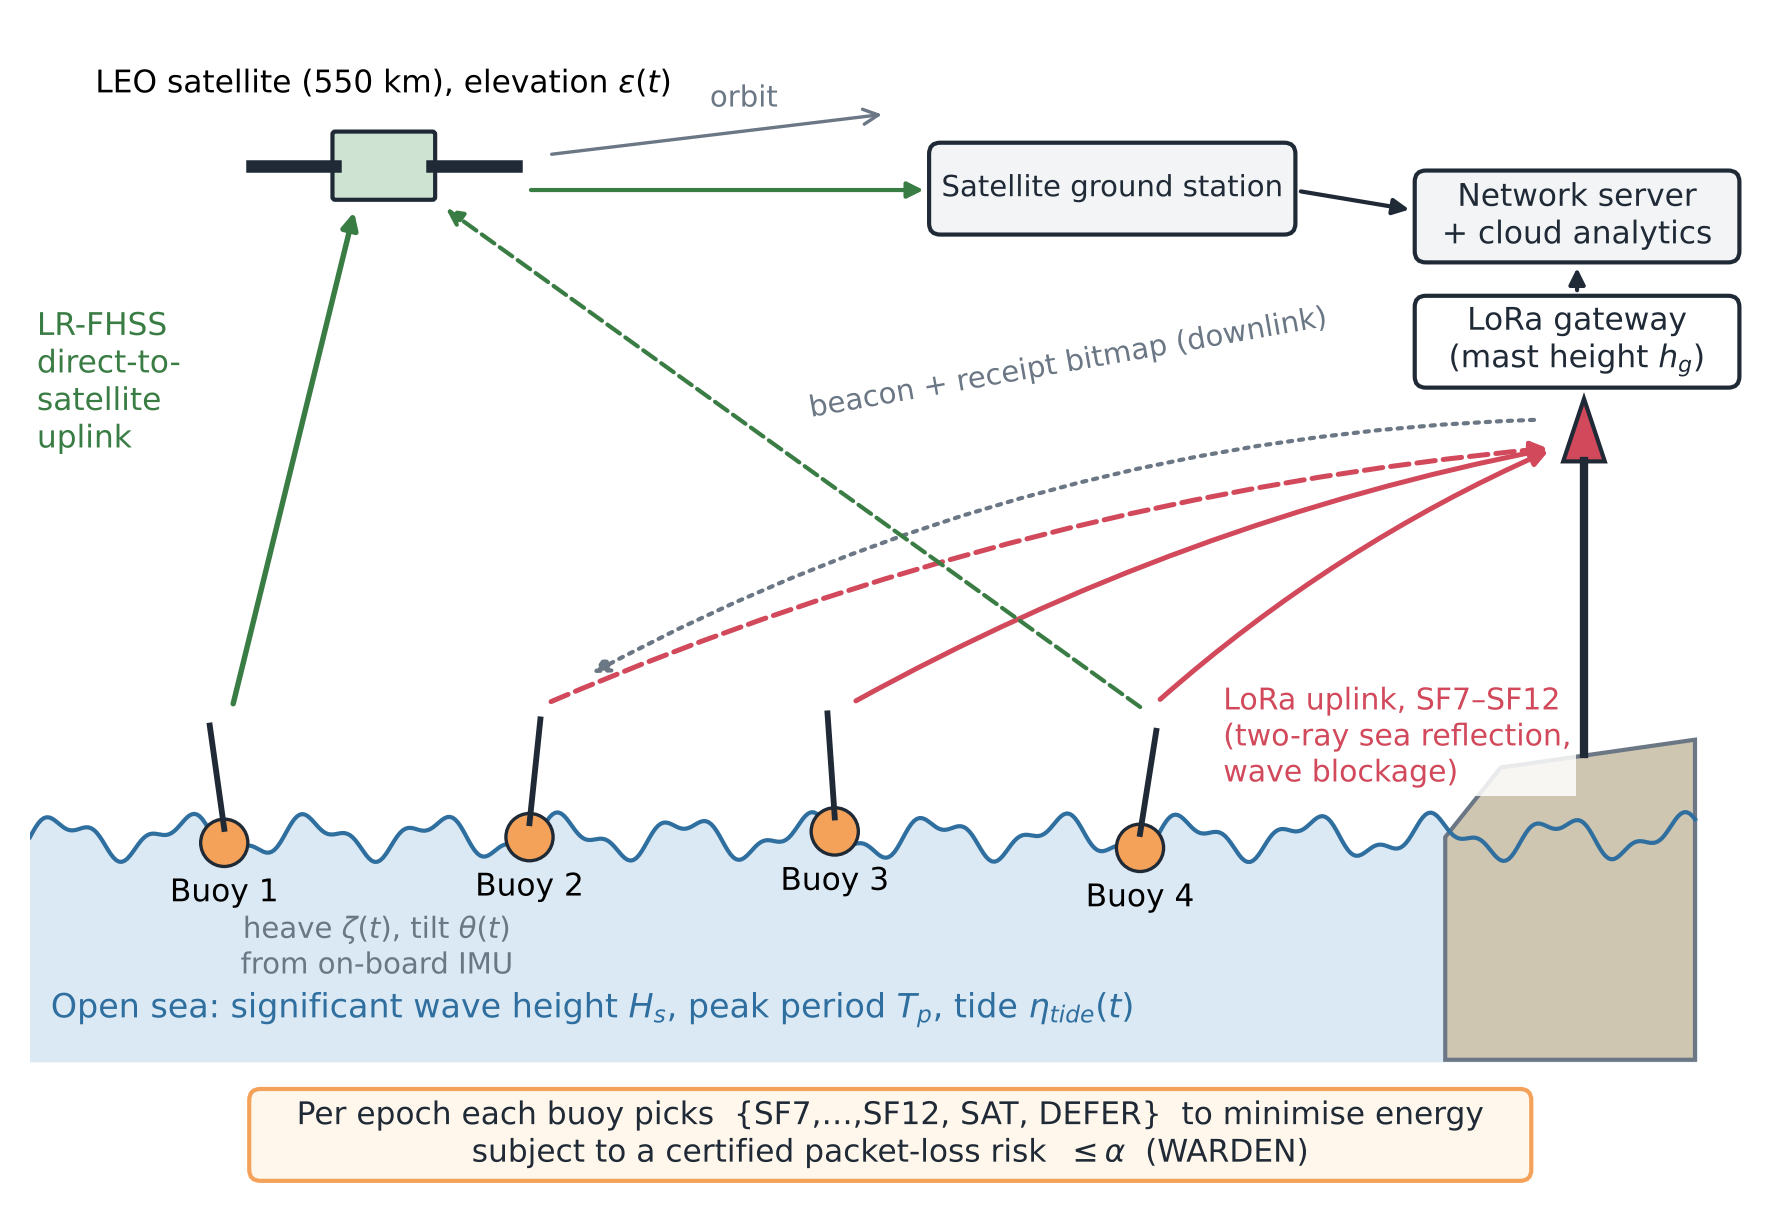
\includegraphics[width=0.95\textwidth,height=\textheight]{../figures/fig1_system_network.png}
\caption{\textbf{Fig. 1} Network model: buoys choose per epoch between
LoRa spreading factors towards a mast-mounted gateway, an LR-FHSS uplink
to a passing LEO satellite, or buffering. Wave heave and tilt, tide and
ducting modulate the links.}
\end{figure}

\hypertarget{sea-state-and-buoy-motion}{%
\subsection{3.2 Sea state and buoy
motion}\label{sea-state-and-buoy-motion}}

The sea is described by the significant wave height \(H_s(t)\) and the
peak period \(T_p(t)\). For a buoy that follows the surface, the
vertical displacement (heave) is modelled as a zero-mean Gaussian
process whose standard deviation follows from the definition of \(H_s\):

\[\zeta_n(t)\sim\mathcal{N}\!\left(0,\;(H_s(t)/4)^2\right). \tag{1}\]

Hull tilt scales with the wave slope. With peak wavelength
\(L_p=gT_p^2/(2\pi)\) and a hull response factor \(\kappa_b\),

\[\theta_{\mathrm{rms}}(t)=\kappa_b\,\frac{\pi H_s(t)}{\sqrt{2}\,L_p(t)},\qquad \theta_n(t)=|\theta_{\mathrm{rms}}(t)\,u|,\;u\sim\mathcal{N}(0,1). \tag{2}\]

The buoy IMU provides noisy estimates
\(\hat H_s,\hat T_p,\hat\theta_{\mathrm{rms}}\) over the beacon window;
these are the only sea-state quantities available to the decision
engine.

\hypertarget{terrestrial-lora-link-over-the-sea}{%
\subsection{3.3 Terrestrial LoRa link over the
sea}\label{terrestrial-lora-link-over-the-sea}}

The instantaneous antenna heights are \(h_b(t)=h_0+\zeta_n(t)\) for the
buoy and \(h_g(t)=\bar h_g+A_{\mathrm{tide}}\sin(2\pi t/T_{M2}+\phi)\)
for the gateway, where the semidiurnal tide (\(T_{M2}=12.42\) h) changes
the mast height above the water. The direct and sea-reflected rays
differ in phase by

\[\Delta\varphi(t)=\frac{4\pi h_g(t)\,h_b(t)}{\lambda d_n}. \tag{3}\]

At the small grazing angle \(\psi\approx(h_g+h_b)/d_n\) the reflection
coefficient \(\Gamma\) is close to \(-1\); surface roughness reduces the
coherent reflection by the Ament factor

\[\rho(t)=\exp\!\left[-8\left(\frac{\pi\sigma_h\sin\psi}{\lambda}\right)^2\right],\qquad \sigma_h=H_s/4. \tag{4}\]

Beyond the radio horizon \(d_h=\sqrt{2kR_E}\,(\sqrt{h_g}+\sqrt{h_b})\) a
diffraction penalty with slope \(\beta\) is added, giving the path loss

\[PL(t)=20\log_{10}\frac{4\pi d_n}{\lambda}-20\log_{10}\left|1+\Gamma\rho(t)e^{-j\Delta\varphi(t)}\right|+\beta\,(d_n-d_h)^{+}. \tag{5}\]

The uplink SNR combines transmit power \(P_t\), the tilted monopole gain
\(G_b(\theta)=2.15+10\log_{10}\cos^2\theta\) dBi, the gateway gain
\(G_g\), a log-normal AR(1) shadowing term \(S(t)\), a ducting gain
\(D(t)\ge 0\), a wave-blockage loss \(B(t)\) that appears when crests
rise above the antenna, Rician fading \(F(t)\) whose K-factor falls with
\(H_s\), and the noise floor \(N_0=-174+10\log_{10}W+NF\):

\[\mathrm{SNR}_L(t)=P_t+G_b(\theta_n)+G_g-PL(t)+S(t)+D(t)-B(t)+F(t)-N_0. \tag{6}\]

A frame sent with spreading factor \(k\) succeeds when the SNR exceeds
the demodulation threshold \(\gamma_k\) and no collision occurs. With
offered background load \(G\) and time on air \(T_k\),

\[Y_k(t)=\mathbb{1}\{\mathrm{SNR}_L(t)\ge\gamma_k\}\cdot\mathbb{1}\{\text{no collision}\},\qquad \Pr[\text{collision}]=1-e^{-2GT_k}. \tag{7}\]

Because \(\gamma_7>\gamma_8>\dots>\gamma_{12}\), the SNR part of (7) is
nested: whenever SF\(k\) succeeds, every larger SF would also have
cleared the threshold. This ordering is exploited by the output head in
Section 4.

\hypertarget{leo-satellite-link}{%
\subsection{3.4 LEO satellite link}\label{leo-satellite-link}}

A LEO satellite at altitude \(h_s\) is visible during passes with
elevation \(\varepsilon(t)\), known on board from ephemeris. The slant
range is

\[r(\varepsilon)=\sqrt{(R_E+h_s)^2-R_E^2\cos^2\varepsilon}-R_E\sin\varepsilon, \tag{8}\]

and the LR-FHSS link margin, with a hemispherical buoy antenna gain
\(G_q(\cdot)\) evaluated at the tilt-corrected elevation, is

\[M_S(t)=P_s+G_q(\varepsilon-\theta_n)+G_{\mathrm{sat}}-20\log_{10}\frac{4\pi r(\varepsilon)}{\lambda}-L_a-P_{\mathrm{sens}}+F_S(t). \tag{9}\]

The satellite frame succeeds when \(M_S\ge 0\), it is not lost to the
Doppler rate at low elevation (probability \(p_D(\varepsilon)\), after
{[}17{]}) and it does not collide with other DtS users.

\hypertarget{energy-model}{%
\subsection{3.5 Energy model}\label{energy-model}}

The energy of one attempt is the radio's electrical power multiplied by
the time on air,

\[E_a=P_{\mathrm{elec}}(a)\,T_a,\qquad E_\varnothing=0, \tag{10}\]

with the standard LoRa time on air for payload \(L\) bytes, bandwidth
\(W\) and coding rate \(CR\):

\[T_k=\left(n_p+4.25\right)\frac{2^k}{W}+\left[8+\max\!\left(\left\lceil\frac{8L-4k+44}{4(k-2\,DE)}\right\rceil(CR+4),0\right)\right]\frac{2^k}{W}. \tag{11}\]

For a 20-byte payload this gives 8.5 mJ at SF7, 197.8 mJ at SF12 and 780
mJ for a 2-s LR-FHSS frame at 22 dBm, a ratio of almost 1:100 between
the cheapest and the most expensive action.

\hypertarget{problem-statements}{%
\subsection{3.6 Problem statements}\label{problem-statements}}

The analysis above leads to five concrete problem statements.

\begin{itemize}
\tightlist
\item
  \textbf{P1 (wave-coupled non-stationarity).} Through (1)--(6) the link
  budget depends on \(H_s\), \(T_p\), the tide and ducting, so a fixed
  SNR margin is too generous in calm water and too optimistic in rough
  water.
\item
  \textbf{P2 (heterogeneous action costs).} Actions differ by two orders
  of magnitude in energy (10), and the satellite action exists only
  during passes (8)--(9).
\item
  \textbf{P3 (unquantified reliability).} Existing learned link
  predictors output point estimates or uncalibrated scores; a buoy
  cannot tell how often its decisions will fail.
\item
  \textbf{P4 (distribution shift).} Storms, hardware changes and new
  sites shift the joint distribution of inputs and outcomes after
  deployment.
\item
  \textbf{P5 (deadline pressure).} A reading that cannot be delivered
  within the buffer age limit is lost, so a policy that is safe on
  average may still discard data that are about to expire.
\end{itemize}

\hypertarget{research-gap}{%
\subsection{3.7 Research gap}\label{research-gap}}

The literature reviewed in Section 2 leaves five gaps. \textbf{G1:}
learned LoRa link adaptation, including maritime deep reinforcement
learning {[}25--27{]}, optimises average reward and gives no bound on
how often its decisions fail. \textbf{G2:} on-board motion data have
been used to predict received power {[}28{]}, but not to condition a
reliability guarantee or to drive a physical channel prior for a hybrid
LoRa and satellite choice. \textbf{G3:} conformal guarantees in wireless
AI {[}29, 31{]} address prediction sets, not the risk of a sequential,
cost-ordered choice whose loss is non-monotone. \textbf{G4:} guarantees
that hold per sea state and recover after shift have not been studied
for maritime links. \textbf{G5:} no scheme allocates reliability budgets
according to data urgency, so certified schemes either waste energy on
stale data or drop readings that are about to expire.

\hypertarget{motivation-for-selective-prediction-and-formal-problem}{%
\subsection{3.8 Motivation for selective prediction and formal
problem}\label{motivation-for-selective-prediction-and-formal-problem}}

Deferring is the natural abstention option of a buoy: a reading kept in
the buffer can ride on the next successful frame. Link selection is
therefore a selective prediction problem in which abstention trades
latency for reliability and energy. Let \(x_{n,t}\) denote the inputs
available before epoch \(t\) (Section 4.1), \(Y_{n,t}\in\{0,1\}^{7}\)
the success indicators of the seven transmit actions, and
\(b(x)\in\{\text{calm},\text{moderate},\text{rough}\}\) the sea-state
stratum given by \(\hat H_s<1\) m, \(1\le\hat H_s<2\) m and
\(\hat H_s\ge 2\) m. For a policy \(\pi\) the attempt-failure loss and
its risk are

\[\ell(\pi;x,Y)=\mathbb{1}\{\pi(x)\ne\varnothing\}\,\left(1-Y_{\pi(x)}\right),\qquad R_b(\pi)=\mathbb{E}\left[\ell(\pi;x,Y)\mid b(x)=b\right]. \tag{12}\]

WARDEN seeks the policy of least expected energy subject to a
per-stratum risk budget that holds with high confidence over the
randomness of the calibration data:

\[\min_{\pi}\;\mathbb{E}\left[E_{\pi(x)}\right]\quad\text{s.t.}\quad \Pr\left[R_b(\pi)\le\alpha\right]\ge 1-\delta,\;\;\forall b. \tag{13}\]

Problem (13) is solved within the threshold family

\[\pi_{\boldsymbol\lambda}(x)=\begin{cases}\min\{a\in\mathcal{A}_t\setminus\{\varnothing\}:s_a(x)\ge\lambda_{b(x)}\}, & \text{if the set is non-empty},\\ \varnothing, & \text{otherwise},\end{cases} \tag{14}\]

where actions are ordered by energy, \(\mathcal{A}_t\) excludes SAT
outside passes and \(s_a(x)\) is the calibrated, uncertainty-penalised
success score of Section 4.3. Raising \(\lambda_b\) moves the choice
towards more robust actions or towards deferral; it does not make the
loss monotone, because a more robust action can still fail on a given
draw. This is why Learn-then-Test {[}34{]}, rather than conformal risk
control for monotone losses {[}33{]}, is used.

\needspace{16\baselineskip}

\textbf{Table 2} Main symbols

\begin{longtable}[]{@{}
  >{\raggedright\arraybackslash}p{(\columnwidth - 2\tabcolsep) * \real{0.3000}}
  >{\raggedright\arraybackslash}p{(\columnwidth - 2\tabcolsep) * \real{0.7000}}@{}}
\toprule\noalign{}
\begin{minipage}[b]{\linewidth}\raggedright
Symbol
\end{minipage} & \begin{minipage}[b]{\linewidth}\raggedright
Meaning
\end{minipage} \\
\midrule\noalign{}
\endhead
\bottomrule\noalign{}
\endlastfoot
\(N\), \(n\), \(t\), \(\Delta\) & number of buoys, buoy index, epoch
index, epoch length (10 min) \\
\(H_s,\;T_p,\;L_p\) & significant wave height, peak period, peak
wavelength \\
\(\zeta,\;\theta,\;\kappa_b\) & heave, tilt, hull response factor \\
\(\hat H_s,\hat T_p,\hat\theta_{\mathrm{rms}}\) & IMU estimates of the
sea state \\
\(h_b,\;h_g,\;A_{\mathrm{tide}}\) & buoy antenna height, gateway height
above sea, tidal amplitude \\
\(d_n,\;d_h,\;\lambda\) & buoy--gateway distance, radio horizon,
wavelength \\
\(\Gamma,\;\rho,\;\psi\) & sea reflection coefficient, roughness factor,
grazing angle \\
\(S,\;D,\;B,\;F\) & shadowing, ducting gain, wave blockage, small-scale
fading (dB) \\
\(\gamma_k,\;T_k\) & SNR threshold and time on air of SF\(k\) \\
\(\varepsilon,\;r(\varepsilon),\;M_S\) & satellite elevation, slant
range, LR-FHSS link margin \\
\(\mathcal{A}\), \(a\), \(\varnothing\) & action set, action, defer
action \\
\(E_a\) & energy of action \(a\) \\
\(Y\in\{0,1\}^7\) & per-action success indicators \\
\(b(x)\) & sea-state stratum \\
\(\mu_a,\;\sigma_a,\;s_a\) & ensemble mean, ensemble spread, penalised
score \\
\(\kappa\) & uncertainty penalty \\
\(\alpha,\;\delta\) & target risk, confidence parameter \\
\(\lambda_b\), \(\Lambda\) & stratum threshold, threshold grid \\
\(\gamma\) & adaptive-conformal step size \\
\(W\), \(d\), \(H\) & history length, embedding width, attention
heads \\
\(\pi_k,\;\ell_k\) & physics-prior success probability of action \(k\)
and its logit \\
\(Q,\;\xi_q,\;w_q\) & Gauss--Hermite order, nodes and weights \\
\(\sigma_r,\;L_B,\;p_B\) & residual spread, blockage loss, blockage
probability in the prior \\
\(\beta_{\mathrm{SF}},\;\beta_{\mathrm{S}}\) & learnable weights of the
physics-residual head \\
\(u_t,\;g,\;A_{\max}\) & urgency flag, guard interval, buffer age
limit \\
\(\alpha_U,\;\rho_U\) & urgent-traffic risk target, share of urgent
epochs \\
\end{longtable}

\hypertarget{proposed-warden-algorithm}{%
\section{4 Proposed WARDEN algorithm}\label{proposed-warden-algorithm}}

WARDEN (Wave-Aware Risk-controlled DEcision eNgine) has three stages,
shown in Fig. 2: input representation with a physics-informed wave
prior, the attention-enhanced predictor, and uncertainty-aware,
urgency-aware risk-controlled selection. Sections 4.1--4.3 describe the
base engine, and Sections 4.4--4.5 the two extensions WARDEN-PI and
WARDEN-U; the full system is denoted WARDEN-PI-U.

\begin{figure}
\centering
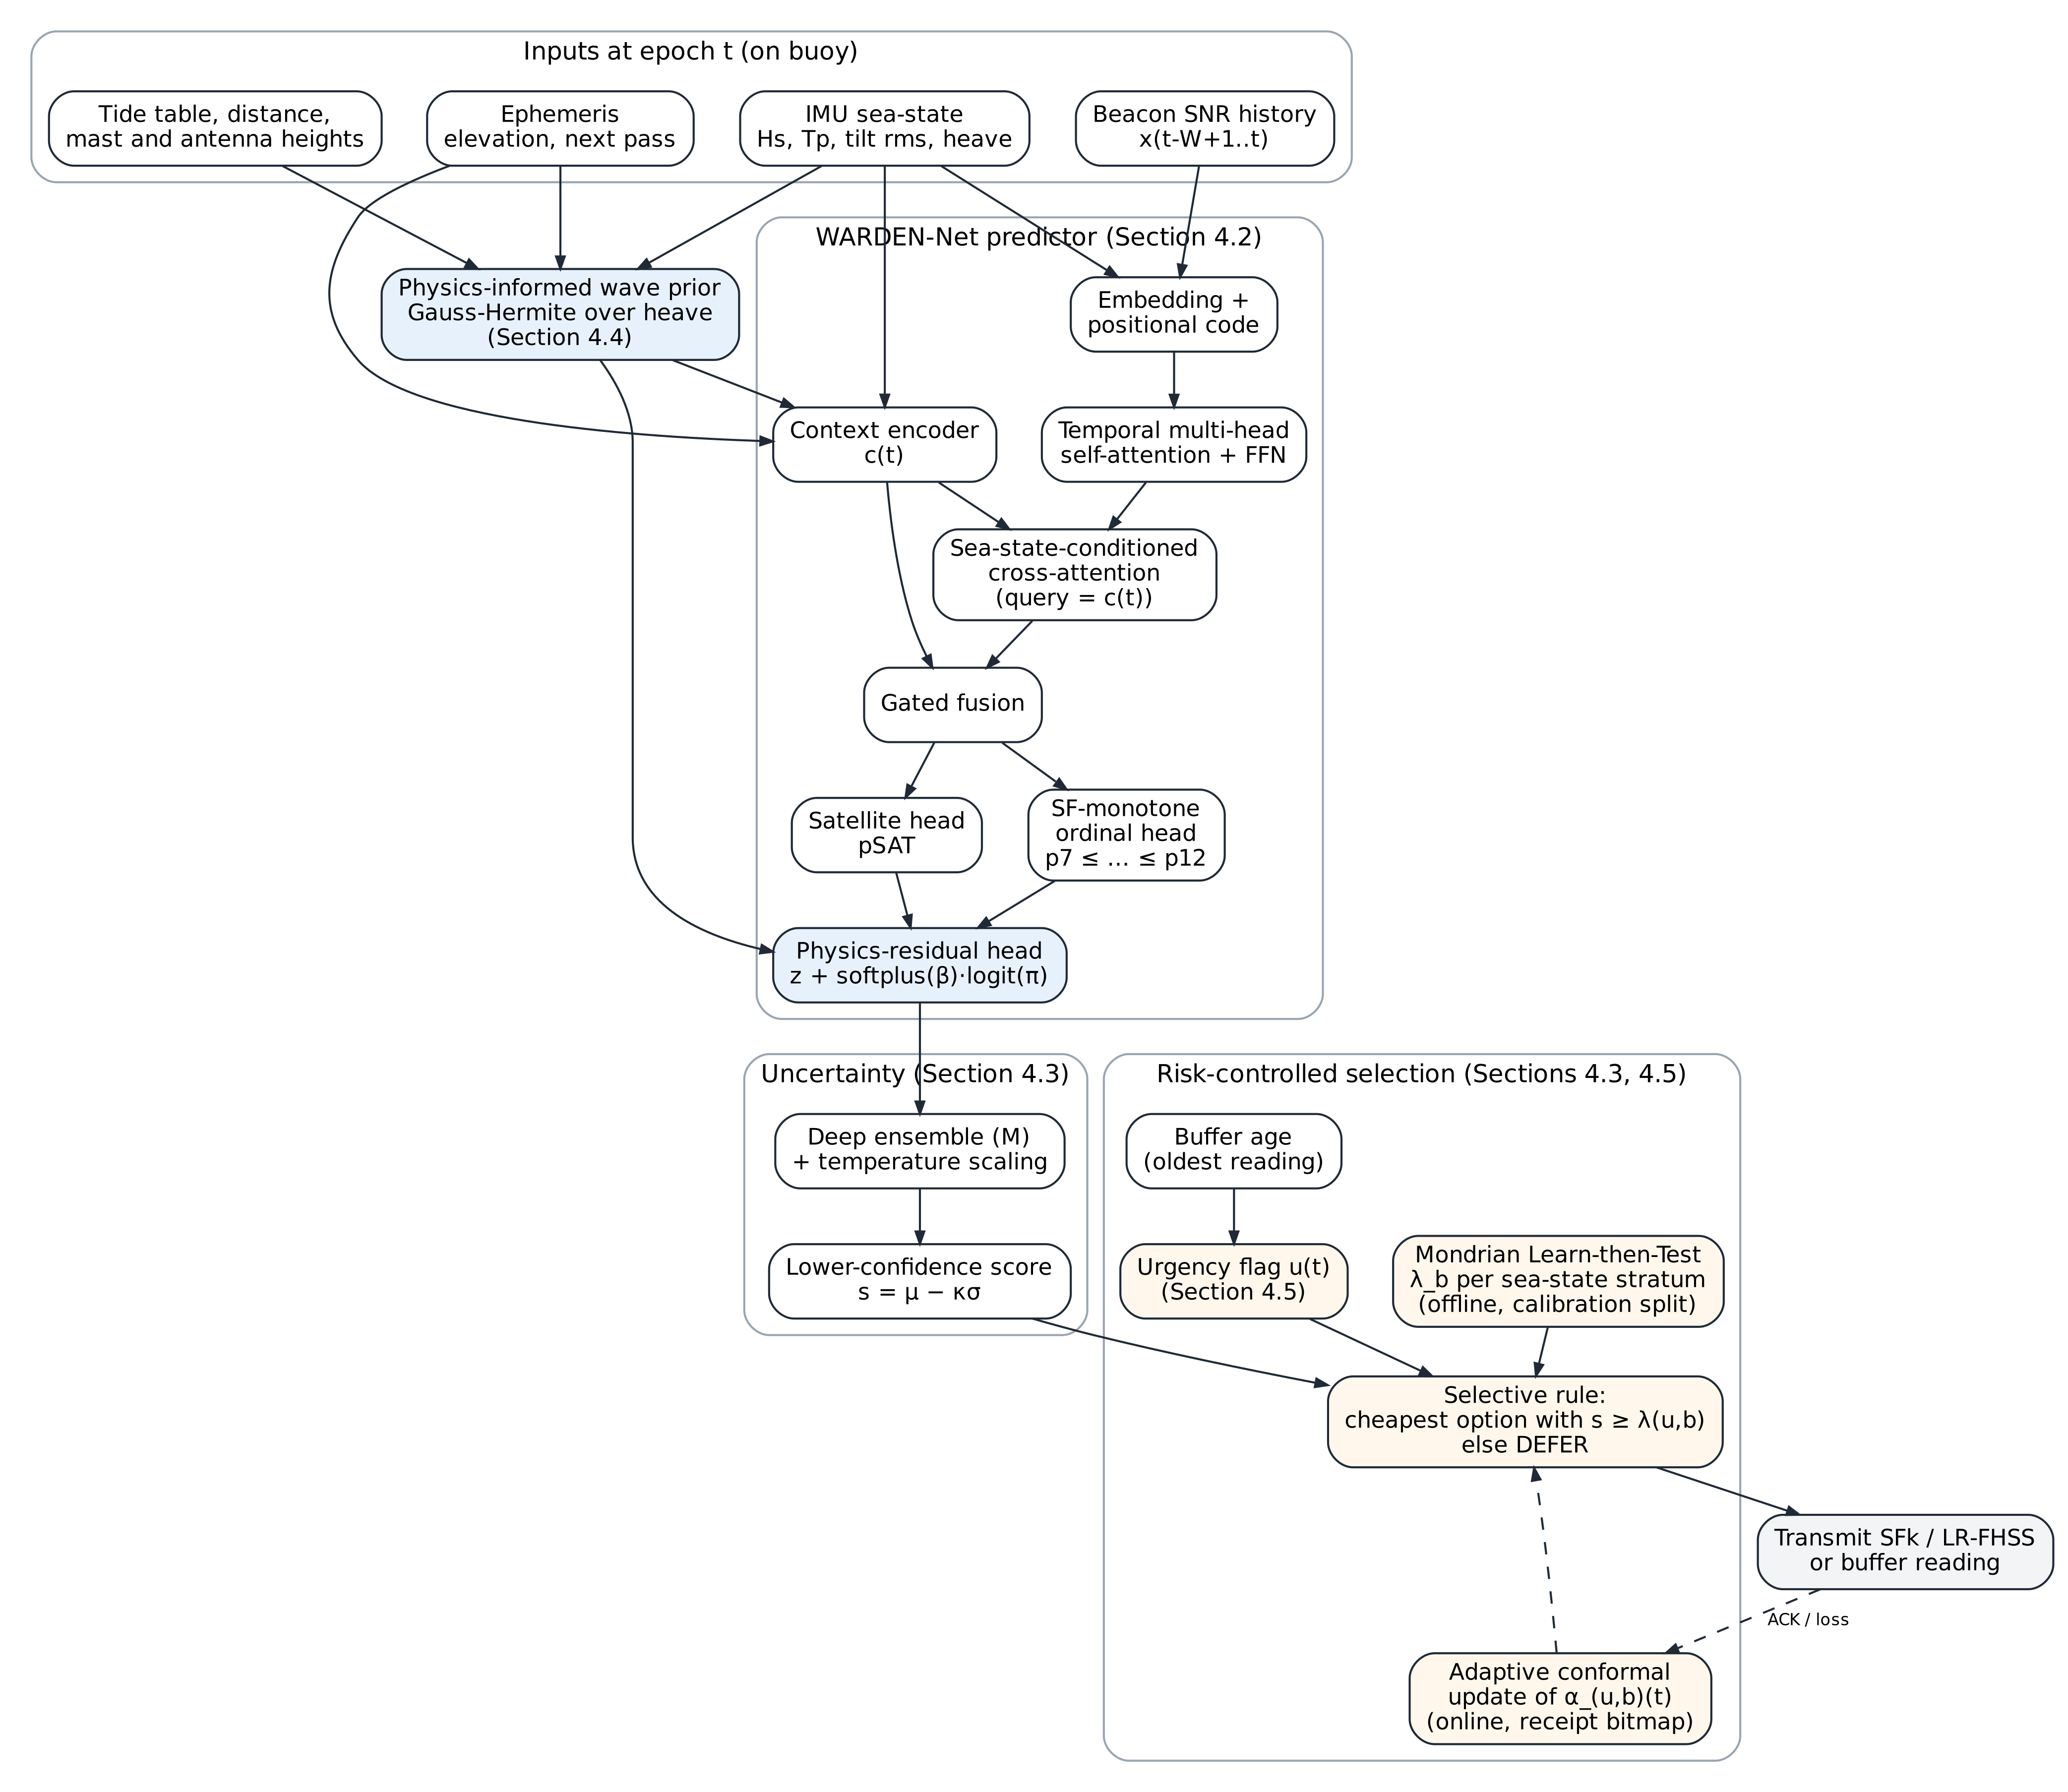
\includegraphics[width=0.92\textwidth,height=\textheight]{../figures/fig2_warden_pipeline.png}
\caption{\textbf{Fig. 2} WARDEN-PI-U pipeline: inputs, physics-informed
wave prior, WARDEN-Net predictor with physics-residual head, uncertainty
quantification, and urgency-aware risk-controlled selection with offline
Mondrian Learn-then-Test calibration and online adaptive conformal
updates.}
\end{figure}

\hypertarget{preprocessing-segmentation-and-input-representation}{%
\subsection{4.1 Preprocessing, segmentation and input
representation}\label{preprocessing-segmentation-and-input-representation}}

\textbf{Segmentation.} The stream of each buoy is cut into sliding
windows of \(W=16\) epochs (2 h 40 min), long enough to span the
decorrelation time of shadowing and about one fifth of a tidal cycle.
Windows end at the beacon of epoch \(t\), so no information from the
decision interval itself leaks into the input.

\textbf{Sequence features.} Each window step \(\tau\) carries a
seven-dimensional vector
\(\mathbf{u}_\tau=[\mathrm{SNR}^{\mathrm{bcn}}_\tau/10,\;m_\tau,\;\hat H_{s,\tau},\;\hat T_{p,\tau}/10,\;\hat\theta_{\mathrm{rms},\tau}/10,\;\hat\zeta_\tau,\;\varepsilon_\tau/90]\),
where \(m_\tau=1\) flags a lost beacon (its SNR is then set to −25 dB).
\textbf{Context features.} The current context
\(\mathbf{c}_t\in\mathbb{R}^{10}\) contains the known distance, antenna
height, current IMU sea state, current elevation and visibility,
time-of-day encoded as \((\sin,\cos)\), and the number of epochs to the
next pass. \textbf{Normalisation.} All features are standardised with
statistics from the training split only. \textbf{Stratum.} The stratum
\(b(x)\) is computed from \(\hat H_s\) in the context vector.

\hypertarget{proposed-attention-enhanced-architecture-warden-net}{%
\subsection{4.2 Proposed attention-enhanced architecture
(WARDEN-Net)}\label{proposed-attention-enhanced-architecture-warden-net}}

\textbf{Temporal encoder.} The window
\(\mathbf{U}\in\mathbb{R}^{W\times 7}\) is embedded and combined with a
learned positional code \(\mathbf{P}\), and one post-norm Transformer
block with \(H=2\) heads is applied:

\[\mathbf{Z}_0=\mathbf{U}\mathbf{W}_e+\mathbf{P},\quad \mathbf{Z}_1=\mathrm{LN}\left(\mathbf{Z}_0+\mathrm{MHA}(\mathbf{Z}_0,\mathbf{Z}_0)\right),\quad \mathbf{Z}=\mathrm{LN}\left(\mathbf{Z}_1+\mathrm{FFN}(\mathbf{Z}_1)\right), \tag{15}\]

with
\(\mathrm{MHA}(\mathbf{Q},\mathbf{K})=[\mathrm{softmax}(\mathbf{Q}\mathbf{W}^q_h(\mathbf{K}\mathbf{W}^k_h)^{\top}/\sqrt{d/H})\,\mathbf{K}\mathbf{W}^v_h]_{h=1}^{H}\mathbf{W}^o\).

\textbf{Sea-state-conditioned cross attention.} The context is encoded
as
\(\mathbf{e}=\mathrm{GELU}(\mathbf{c}\mathbf{W}_{c1})\mathbf{W}_{c2}\)
and used as the \emph{query} over the encoded history:

\[\mathbf{z}=\mathrm{MHA}(\mathbf{e},\mathbf{Z})\in\mathbb{R}^{d}. \tag{16}\]

Under calm water the query can emphasise the latest beacons, which track
slow shadowing and ducting; in rough water it can spread weight over the
window to average out wave-induced fluctuations. Section 7 shows that
the learned attention indeed differs by stratum.

\textbf{Gated fusion.} A context-dependent gate decides how much history
to trust:

\[\mathbf{v}=\mathrm{GELU}\!\left(\left[\mathbf{z}\odot\sigma(\mathbf{e}\mathbf{W}_g+\mathbf{b}_g)+\mathbf{e}\right]\mathbf{W}_h\right). \tag{17}\]

\textbf{SF-monotone ordinal head.} Following the nesting noted after
(7), the SF logits are built as a base logit plus cumulative
non-negative increments, and a separate head models the satellite:

\[z_{7}=\mathbf{v}^{\top}\mathbf{w}_0,\qquad z_{k}=z_{7}+\sum_{j=8}^{k}\mathrm{softplus}(\mathbf{v}^{\top}\mathbf{w}_j),\;k=8,\dots,12,\qquad z_{\mathrm{S}}=\mathbf{v}^{\top}\mathbf{w}_{\mathrm{S}}. \tag{18}\]

Hence \(p_7\le p_8\le\dots\le p_{12}\) by construction, which prevents
physically impossible rankings that would otherwise confuse the
cost-ordered rule (14).

\textbf{Training loss.} All seven outputs are trained jointly with a
masked binary cross-entropy in which the satellite term is active only
during passes (\(v_t=1\)):

\[\mathcal{L}=\frac{1}{\sum_i\sum_a\omega_{ia}}\sum_i\sum_{a}\omega_{ia}\left[\log(1+e^{z_{ia}})-Y_{ia}z_{ia}\right],\qquad \omega_{ia}=\begin{cases}v_{i},&a=\mathrm{SAT}\\1,&\text{otherwise.}\end{cases} \tag{19}\]

In the testbed all actions are labelled in every epoch because the
simulator evaluates counterfactual outcomes; in a deployment the same
labels are obtained from periodic probe frames during a commissioning
period (Section 8).

\hypertarget{uncertainty-estimation-calibration-and-risk-controlled-selective-prediction}{%
\subsection{4.3 Uncertainty estimation, calibration and risk-controlled
selective
prediction}\label{uncertainty-estimation-calibration-and-risk-controlled-selective-prediction}}

\textbf{Ensemble and temperature scaling.} \(M=3\) WARDEN-Nets with
different initialisations are trained. Each member's logits are divided
by an action-specific temperature fitted on the validation split, and
the calibrated probabilities are averaged:

\[\mu_a(x)=\frac{1}{M}\sum_{m=1}^{M}\sigma\!\left(z^{(m)}_a(x)/T^{(m)}_a\right),\qquad \sigma_a(x)=\mathrm{std}_m\,\sigma\!\left(z^{(m)}_a(x)/T^{(m)}_a\right). \tag{20}\]

\textbf{Penalised score.} Epistemic disagreement is converted into
caution with a lower-confidence score

\[s_a(x)=\mathrm{clip}\left(\mu_a(x)-\kappa\,\sigma_a(x),\,0,\,1\right),\qquad \kappa=1. \tag{21}\]

\textbf{Mondrian Learn-then-Test.} Let \(\mathcal{D}^{\mathrm{cal}}_b\)
be the \(n_b\) calibration epochs of stratum \(b\) and
\(\Lambda=\{\lambda_1>\lambda_2>\dots>\lambda_J\}\) a grid from 0.999
down to 0.30 (\(J=141\)). For each \(\lambda_j\) the empirical risk of
policy (14) is

\[\hat R_b(\lambda_j)=\frac{1}{n_b}\sum_{i\in\mathcal{D}^{\mathrm{cal}}_b}\ell(\pi_{\lambda_j};x_i,Y_i). \tag{22}\]

Because the loss is binary, the null hypothesis
\(H_{b,j}:R_b(\lambda_j)>\alpha\) is tested with the exact binomial
p-value

\[p_{b,j}=\Pr\left[\mathrm{Bin}(n_b,\alpha)\le n_b\hat R_b(\lambda_j)\right]. \tag{23}\]

Hypotheses are tested in the fixed order \(j=1,2,\dots\) (most
conservative first), and the threshold is the last rejected one:

\[\hat\lambda_b=\lambda_{\hat j},\qquad \hat j=\max\{j:\;p_{b,1}\le\delta,\dots,p_{b,j}\le\delta\}, \tag{24}\]

with \(\hat\lambda_b=1.01\) (always defer) when \(p_{b,1}>\delta\).

\textbf{Proposition 1 (per-stratum risk certificate).} If the
calibration and test epochs within stratum \(b\) are exchangeable and
the predictor is fixed before calibration, then

\[\Pr\left[R_b(\pi_{\hat\lambda_b})\le\alpha\right]\ge 1-\delta\quad\text{for every stratum } b. \tag{25}\]

\emph{Proof sketch.} Fixed-sequence testing of \(H_{b,1},H_{b,2},\dots\)
at level \(\delta\) controls the family-wise error rate at \(\delta\)
without any monotonicity assumption, because a false rejection can occur
only at the first true null in the sequence {[}34{]}. The p-values (23)
are valid under exchangeability since \(n_b\hat R_b(\lambda_j)\) is
binomial with success probability \(R_b(\lambda_j)\). Stratification is
a Mondrian partition: conditioning on \(b\) preserves exchangeability
within each cell, so the argument holds separately for each \(b\).
\(\square\)

\textbf{Online adaptive conformal update.} Exchangeability is broken by
storms and site changes. During operation each stratum keeps a working
level \(\alpha_{b,t}\), initialised at \(\alpha\), and maps it to the
most aggressive threshold whose calibration risk curve stays below it in
the same fixed order; the receipt bitmap then supplies the realised loss
\(\mathrm{err}_t\) of the previous attempt and

\[\alpha_{b,t+1}=\mathrm{clip}\left(\alpha_{b,t}+\gamma(\alpha-\mathrm{err}_t),\,10^{-4},\,0.5\right),\qquad \gamma=0.005. \tag{26}\]

Following Gibbs and Candès {[}35{]}, without clipping the update
guarantees, for any sequence of data,

\[\left|\frac{1}{T_b}\sum_{t=1}^{T_b}\mathrm{err}_t-\alpha\right|\le\frac{\max(\alpha_{b,1},1-\alpha_{b,1})+\gamma}{\gamma\,T_b}, \tag{27}\]

so the long-run failure frequency in each stratum converges to
\(\alpha\) at rate \(O(1/T_b)\). Clipping at 0.5 is inactive in all our
runs except the first epochs after an abrupt shift. Algorithms 1 and 2
summarise the offline and online stages; Algorithm 2 already includes
the extensions of Sections 4.4 and 4.5.

\textbf{Algorithm 1} WARDEN offline training and certification

\begin{verbatim}
Input : training, validation and calibration splits; α, δ, κ, grid Λ
1  standardise features with training statistics
2  for m = 1..M: train WARDEN-Net_m with loss (19); fit temperatures T_a^(m) on validation
3  for each calibration epoch i: compute μ, σ by (20) and s by (21)
4  for each stratum b:
5      for j = 1..J (λ_1 > … > λ_J):
6          compute R̂_b(λ_j) by (22) and p_{b,j} by (23)
7          if p_{b,j} > δ: break
8      λ̂_b ← last λ_j with p_{b,j} ≤ δ (1.01 if none)
9      store the calibration risk curve R̂_b(·)
Output: ensemble, temperatures, {λ̂_b}, {R̂_b(·)}
\end{verbatim}

\textbf{Algorithm 2} WARDEN-PI-U online operation on buoy n

\begin{verbatim}
1   α_{u,b} ← α (u = 0) or α_U (u = 1) for all cells
2   every epoch t:
3       receive beacon; read SNR and receipt bit err_{t-1}
4       update the level of the previous epoch's cell (u,b) by (32)
5       read IMU sea state, tide table, ephemeris; build window and context
6       compute physics prior π by (28)-(29)
7       b ← stratum(Ĥ_s);  u ← urgency flag by (31)
8       λ ← most aggressive λ_j with R̂_b(λ_1..λ_j) ≤ α_{u,b}
9       compute s_a for available actions by (20), (21), (30)
10      a* ← cheapest action with s_a ≥ λ, otherwise ∅           # rule (14)
11      if a* = ∅: buffer reading (drop readings older than A_max)
12      else: send buffered readings with action a*
\end{verbatim}

\hypertarget{physics-informed-wave-prior-and-residual-head-warden-pi}{%
\subsection{4.4 Physics-informed wave prior and residual head
(WARDEN-PI)}\label{physics-informed-wave-prior-and-residual-head-warden-pi}}

The buoy knows its distance \(d_n\), antenna height \(h_0\) and mast
height \(\bar h_g\), can read the tide \(h_g(t)\) from tide tables,
measures \(\hat H_s\) and \(\hat\theta_{\mathrm{rms}}\) with its IMU,
and knows the satellite elevation from ephemeris. These quantities are
enough to evaluate the deterministic part of (3)--(9) in closed form.
Let \(\overline{\mathrm{SNR}}(\zeta)\) denote the large-scale SNR (6)
without the unknown shadowing, ducting and fading terms, evaluated at
heave \(\zeta\), mean tilt
\(\bar\theta=\hat\theta_{\mathrm{rms}}\sqrt{2/\pi}\) and roughness
\(\sigma_h=\hat H_s/4\). Integrating the heave distribution (1) with
\(Q\)-point Gauss--Hermite quadrature (nodes \(\xi_q\), normalised
weights \(w_q\), \(Q=10\)) gives the wave-averaged success prior of
SF\(k\):

\[\pi_k(x)=(1-p_B)\sum_{q=1}^{Q}w_q\,\Phi\!\left(\frac{\overline{\mathrm{SNR}}(\xi_q\hat H_s/4)-\gamma_k}{\sigma_r}\right)+p_B\sum_{q=1}^{Q}w_q\,\Phi\!\left(\frac{\overline{\mathrm{SNR}}(\xi_q\hat H_s/4)-L_B-\gamma_k}{\sigma_r}\right), \tag{28}\]

where \(\Phi\) is the standard normal distribution function,
\(\sigma_r=4.5\) dB lumps the residual variability the buoy cannot
compute, \(L_B\) is the mean blockage loss and \(p_B\) the blockage
probability implied by \(\hat H_s\) and \(h_0\) {[}8{]}. For the
satellite,

\[\pi_{\mathrm{S}}(x)=\mathbb{1}\{\varepsilon>0\}\,\Phi\!\left(\frac{M_S(\varepsilon,\bar\theta)}{\sigma_s}\right)\left(1-p_D(\varepsilon)\right)\left(1-p_c\right), \tag{29}\]

with \(M_S\) from (9) without fading and \(p_c\) the nominal collision
probability. Because \(\gamma_7>\dots>\gamma_{12}\), the prior satisfies
\(\pi_7\le\dots\le\pi_{12}\) automatically.

The prior enters WARDEN-Net twice. Its logits
\(\boldsymbol{\ell}=\mathrm{logit}(\boldsymbol\pi)\) and the expected
SNR are appended to the context vector \(\mathbf{c}_t\), so that the
cross-attention query of (16) is informed by physics. In addition, the
output logits of (18) are replaced by a \emph{physics-residual head}

\[\tilde z_k=z_k+\mathrm{softplus}(\beta_{\mathrm{SF}})\,\ell_k,\quad k=7,\dots,12,\qquad \tilde z_{\mathrm{S}}=z_{\mathrm{S}}+\mathrm{softplus}(\beta_{\mathrm{S}})\,\ell_{\mathrm{S}}, \tag{30}\]

with learnable scalars \(\beta_{\mathrm{SF}},\beta_{\mathrm{S}}\). A
single shared \(\beta_{\mathrm{SF}}\ge0\) preserves the SF ordering of
(18), and the network only has to learn what physics leaves unexplained:
shadowing, ducting, interference and modelling error. If the prior is
wrong, the network can shrink \(\beta\), and the certification layer
still enforces the risk target (Section 7.4). Evaluating (28)--(29)
costs \(7Q\) link-budget evaluations, about \(10^3\) operations per
epoch.

\hypertarget{urgency-aware-mondrian-certification-warden-u}{%
\subsection{4.5 Urgency-aware Mondrian certification
(WARDEN-U)}\label{urgency-aware-mondrian-certification-warden-u}}

A reading whose age approaches the buffer limit \(A_{\max}\) is lost if
the buoy keeps deferring. WARDEN-U therefore refines the Mondrian
partition with an urgency flag

\[u_t=\mathbb{1}\{t-t^{\mathrm{old}}_{n}\ge A_{\max}-g\}, \tag{31}\]

where \(t^{\mathrm{old}}_n\) is the arrival epoch of the oldest buffered
reading and \(g\) a guard interval (\(g=3\) epochs). Each cell \((u,b)\)
keeps its own working level \(\alpha_{u,b,t}\) and its own target,
\(\alpha\) for ordinary epochs and \(\alpha_U\) for urgent ones, updated
as in (26):

\[\alpha_{u,b,t+1}=\mathrm{clip}\left(\alpha_{u,b,t}+\gamma\,(\alpha^{(u)}-\mathrm{err}_t),\,10^{-4},\,0.6\right),\qquad \alpha^{(0)}=\alpha,\;\alpha^{(1)}=\alpha_U. \tag{32}\]

By (27), applied to each cell, the long-run failure frequency of
ordinary traffic converges to \(\alpha\) and that of urgent traffic to
\(\alpha_U\). The operator thus states two numbers, the reliability of
routine transmissions and the extra risk accepted to rescue data that
would otherwise expire, and the overall failure rate is the
urgency-weighted mixture

\[R=(1-\rho_U)\,R^{(0)}+\rho_U\,R^{(1)},\qquad \rho_U=\Pr[u_t=1]. \tag{33}\]

Because urgent epochs are rare, (33) stays close to \(\alpha\) even when
\(\alpha_U\) is larger. Separating the cells also has a subtler benefit,
visible even with \(\alpha_U=\alpha\): the update no longer averages the
very different failure statistics of fresh and nearly expired buffers,
so each cell's threshold adapts to its own conditions.

\textbf{Complexity.} WARDEN-Net has 17 229 parameters (17 487 with the
physics-residual head). One forward pass costs \(O(W^2d+Wd^2)\)
operations, of the order of \(10^5\) multiply-accumulate operations for
\(W=16\), \(d=32\), so a three-member ensemble needs well under 1 MFLOP
per decision, within reach of a Cortex-M4-class microcontroller every 10
min. Online calibration costs one table look-up and one addition per
epoch.

\hypertarget{baselines-and-experimental-setup}{%
\section{5 Baselines and experimental
setup}\label{baselines-and-experimental-setup}}

\hypertarget{sandbox-and-test-bed}{%
\subsection{5.1 Sandbox and test bed}\label{sandbox-and-test-bed}}

All experiments run in a software sandbox test bed that implements the
models of Section 3 in Python (NumPy, SciPy, scikit-learn) with a
purpose-written automatic-differentiation engine, so that every number
in this paper can be regenerated on a laptop without a GPU. The test bed
is synthetic: it is a physics-guided emulator, not a sea trial, and its
parameters (Table 3) were chosen from published offshore and DtS studies
{[}5, 8, 15--19{]}. Each deployment contains \(N=20\) buoys with
distances drawn uniformly in 5--32 km and antenna heights in 0.8--1.5 m,
observed for 60 days at 10-min epochs (8 640 epochs per buoy). The
regional sea state follows a log-AR(1) process with Poisson storm
events; each buoy adds a local perturbation. For every epoch the
ground-truth success probability of every action is computed from 32
Monte Carlo draws of wave phase, blockage and fading, and one draw
provides the observed labels.

\needspace{16\baselineskip}

\textbf{Table 3} Test-bed parameters

\begin{longtable}[]{@{}
  >{\raggedright\arraybackslash}p{(\columnwidth - 2\tabcolsep) * \real{0.3000}}
  >{\raggedright\arraybackslash}p{(\columnwidth - 2\tabcolsep) * \real{0.7000}}@{}}
\toprule\noalign{}
\begin{minipage}[b]{\linewidth}\raggedright
Parameter
\end{minipage} & \begin{minipage}[b]{\linewidth}\raggedright
Value
\end{minipage} \\
\midrule\noalign{}
\endhead
\bottomrule\noalign{}
\endlastfoot
Carrier, bandwidth, noise figure & 868 MHz, 125 kHz, 6 dB \\
LoRa \(P_t\), gateway gain, mast height & 14 dBm, 6 dBi, 15 m (10 m in
OOD-B) \\
Tide & M2, amplitude 1.5 m \\
Diffraction slope beyond horizon \(\beta\) & 1.2 dB/km \\
Shadowing & AR(1), \(\rho=0.97\) per epoch, \(\sigma=3\) dB \\
Ducting gain & 0--6 dB, logistic in an AR(1) drive with diurnal and
sea-state terms \\
Rician K (LoRa / satellite) & \(\max(1,10-2H_s)\) dB /
\(\max(2,8-0.8H_s)\) dB \\
SF thresholds \(\gamma_7..\gamma_{12}\) & −7.5, −10, −12.5, −15, −17.5,
−20 dB \\
Background load \(G\) & 0.02 frames/s (0.05 in OOD-B) \\
LEO altitude, mean revisit & 550 km, 95 min, max elevation 12°--90° \\
LR-FHSS power, sensitivity, frame & 22 dBm, −137 dBm, 2.0 s \\
DtS collision probability & 0.08 (0.15 in OOD-B) \\
Radio power draw (14 / 22 dBm) & 0.15 W / 0.39 W \\
Payload, epoch, buffer age limit & 20 bytes, 10 min, 18 epochs (3 h) \\
Hull response \(\kappa_b\), IMU noise & 2.0 (3.0 in OOD-B), 8 \% \\
Sea state, in-distribution & mean \(H_s\) 1.2 m, 0.08 storms/day, storm
peak 2.5--3.5 m \\
Sea state, OOD-A & mean \(H_s\) 1.8 m, 0.15 storms/day, storm peak 4--7
m \\
\end{longtable}

\textbf{Splits.} Splits are chronological to respect temporal
dependence: days 0--36 for training (every second epoch used, 51 680
windows), 36--42 for validation and temperature fitting (17 280), 42--48
for calibration (17 280) and 48--60 for testing (34 560). \textbf{OOD-A}
is a separate deployment with new buoys and severe storms.
\textbf{OOD-B} is a site and hardware shift: lower mast, livelier hull,
heavier interference and a shorter distance range. Two robustness sets
reuse the in-distribution channel realisation with 30 \% IMU noise or 3
dB beacon noise. Every experiment is repeated with three independent
seeds (1, 2, 3), which change the deployment, the network initialisation
and the calibration draw; tables report mean ± standard deviation.

\hypertarget{baselines}{%
\subsection{5.2 Baselines}\label{baselines}}

\emph{Rule-based policies.} (i) \textbf{ADR-\(m\) dB}: an
adaptive-data-rate style rule that picks the smallest SF whose threshold
plus a margin \(m\in\{5,10,15\}\) dB lies below an exponentially
weighted beacon SNR, otherwise the satellite if visible, otherwise SF12;
(ii) \textbf{Always-SF12}; (iii) \textbf{Sat-first}: satellite whenever
visible, otherwise SF12; (iv) \textbf{Oracle}: the cheapest action that
actually succeeds (unattainable lower bound).

\emph{Predictors} (all followed by the same temperature scaling and
selection rule): logistic regression, histogram gradient boosting and a
two-layer MLP on 42 hand-crafted features (last four window steps,
context, SNR mean, minimum, spread and beacon-loss rate); a GRU sequence
model; and a Transformer encoder with mean pooling and concatenated
context, representative of attention channel predictors {[}20--22{]}.
All neural models use width \(d=32\) and Adam with learning rate
\(2\times10^{-3}\), batch 512, up to 8 epochs and early stopping on
validation loss.

\emph{Physics-informed baselines.} (v) \textbf{Physics prior only}: the
closed-form prior (28)--(29) with temperature scaling and the same
certification, i.e.~no learning at all; (vi) \textbf{gradient boosting +
prior}: histogram gradient boosting given the prior logits as extra
features, which tests whether the gain of WARDEN-PI comes from the prior
or from the attention residual design. \emph{Prior misspecification.} To
test robustness to a wrong physics model, WARDEN-PI is also trained and
calibrated with a deliberately biased prior (reflection coefficient
−0.80 instead of −0.95, diffraction slope 0.8 instead of 1.2 dB/km, a +3
m mast-height error, a 3 dB instead of 4.5 dB residual spread, 6 dB
instead of 10.5 dB blockage loss, and a 2 dB optimistic satellite
receiver).

\emph{Selection rules} (with the WARDEN ensemble): a naive threshold of
0.5, the nominal threshold \(1-\alpha\), global (unstratified) LTT,
Mondrian LTT, Mondrian LTT with the online update (26), and the
urgency-aware two-tier rule (31)--(32) with
\(\alpha_U\in\{0.05,0.10,0.20,0.30\}\) and guard \(g=3\).

\hypertarget{metrics}{%
\subsection{5.3 Metrics}\label{metrics}}

Prediction quality is measured by the mean AUROC over actions, the Brier
score and the expected calibration error (ECE, 15 bins). Decision
quality is measured by the realised attempt-failure risk overall and per
stratum, the deferral rate, the reading delivery ratio (RDR, the
fraction of readings that reach the gateway within the 3-h buffer
limit), the mean latency of delivered readings and the energy per
delivered reading. Unless stated otherwise \(\alpha=0.05\) and
\(\delta=0.1\).

\hypertarget{quantitative-results}{%
\section{6 Quantitative results}\label{quantitative-results}}

All results are means ± standard deviations over three seeds, computed
on the held-out test days (48--60) or on the out-of-distribution
deployments. Raw per-seed outputs are released with the code.

\hypertarget{test-bed-behaviour}{%
\subsection{6.1 Test-bed behaviour}\label{test-bed-behaviour}}

Figure 3 shows ten days of one buoy at 20 km. Storm episodes raise
\(H_s\) above 2.5 m; the beacon SNR then drops by 5--10 dB and
fluctuates faster, and the true success probability of SF7 collapses
while SF12 degrades more slowly. Satellite opportunities appear as short
bursts whose success probability varies with elevation. These traces
confirm problem statements P1 and P2: the cheapest adequate action
changes within hours and is tied to the sea state.

\begin{figure}
\centering
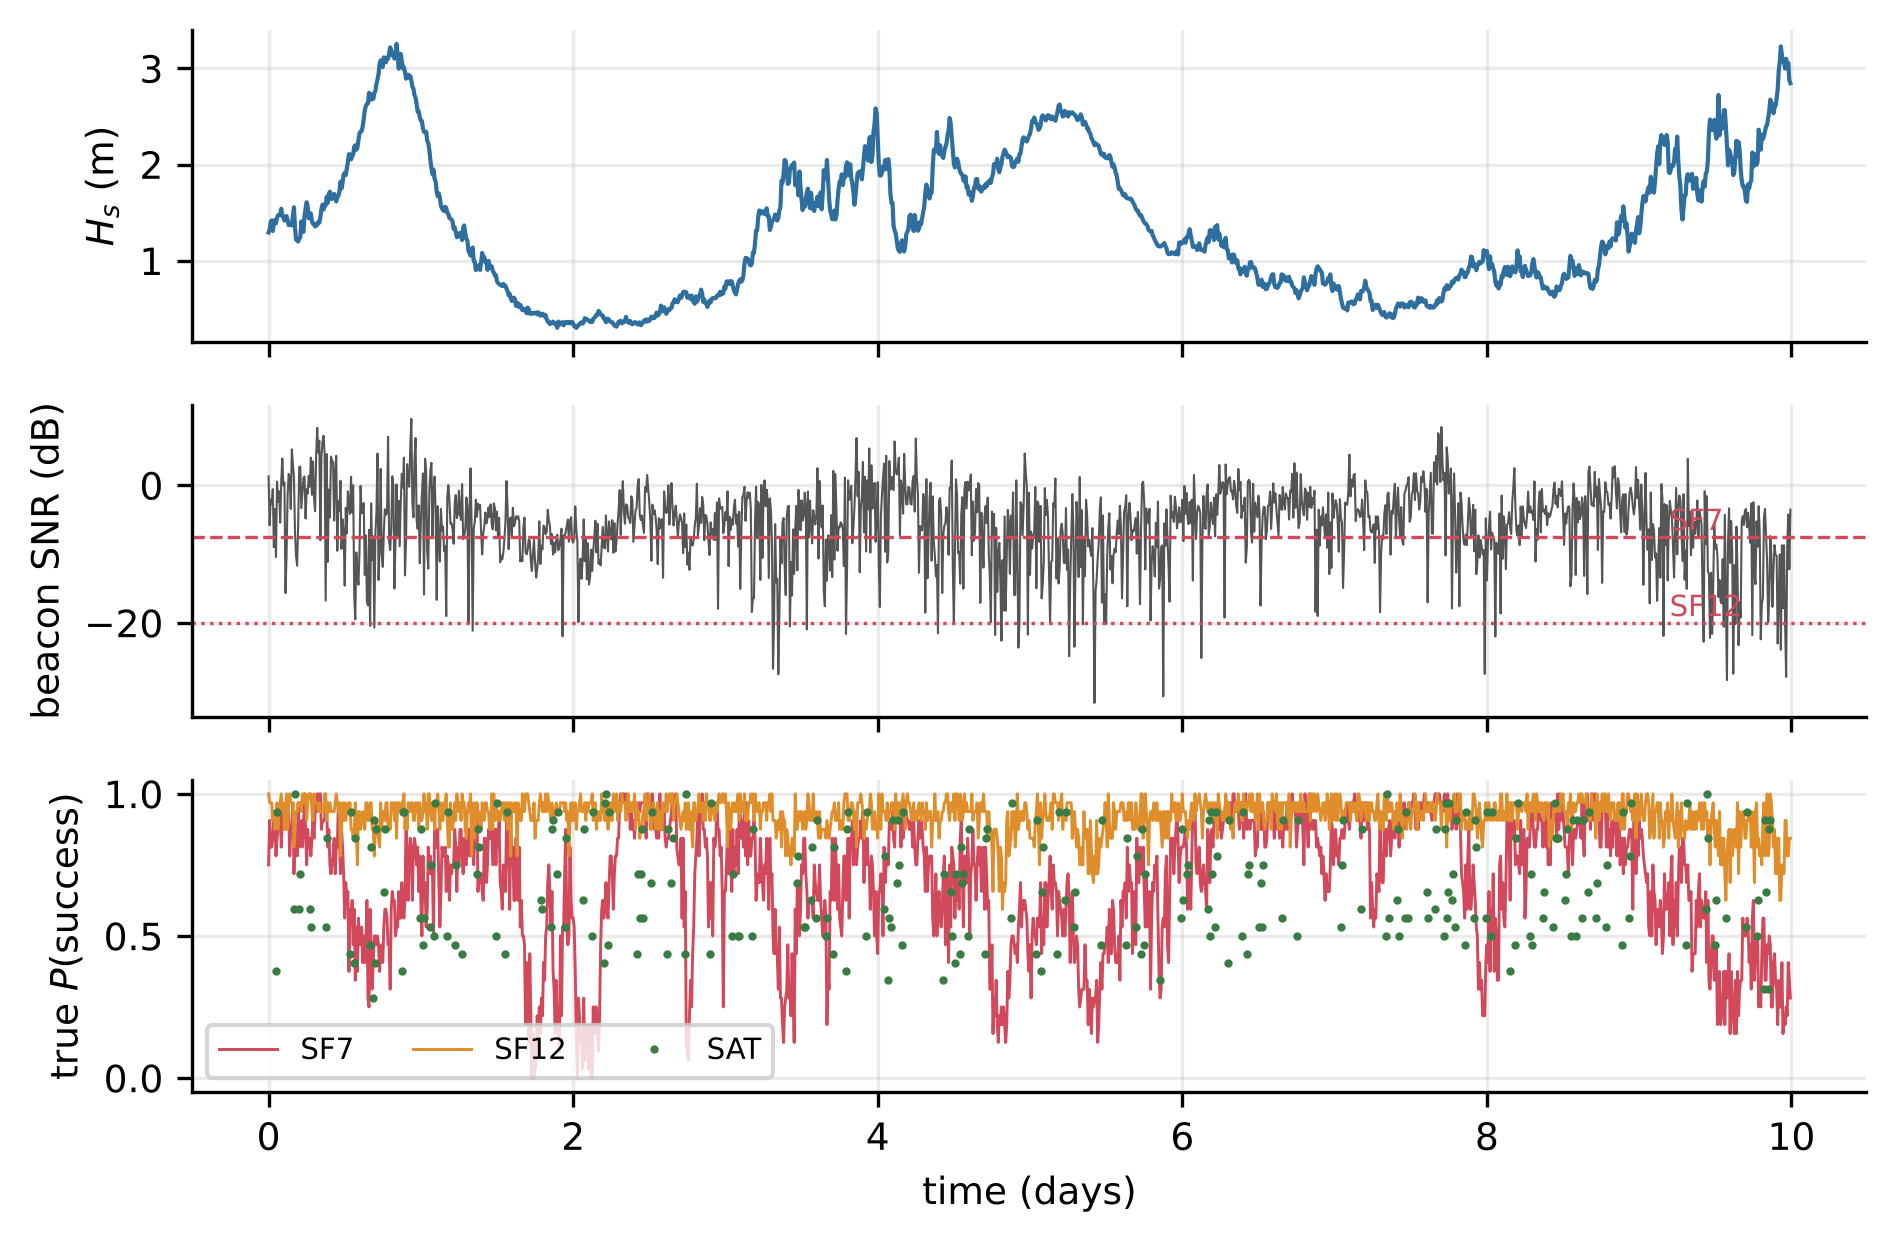
\includegraphics[width=0.95\textwidth,height=\textheight]{../figures/fig3_testbed_traces.png}
\caption{\textbf{Fig. 3} Ten days of one 20-km buoy in the test bed:
significant wave height, beacon SNR with SF7 and SF12 thresholds, and
ground-truth success probability of SF7, SF12 and the satellite action.}
\end{figure}

\hypertarget{prediction-quality}{%
\subsection{6.2 Prediction quality}\label{prediction-quality}}

Table 4 compares the predictors. All models reach similar discrimination
in distribution (AUROC 0.883--0.886), which is expected because much of
the remaining uncertainty is aleatoric (wave phase and fading during the
frame). WARDEN-Net has the lowest Brier score in distribution and under
OOD-A, and its calibration error under the site shift (OOD-B, ECE 0.023)
is lower than that of the Transformer baseline (0.032), gradient
boosting (0.028) and the MLP (0.036), and close to the GRU (0.021). The
differences in Brier score are small, below one per cent in relative
terms, and we do not claim that the attention architecture is a large
accuracy improvement on its own. Its value lies in delivering ordered,
well-calibrated scores to the selection layer, as shown next. Figure 4
confirms that the calibrated WARDEN-Net probabilities lie close to the
diagonal.

\needspace{16\baselineskip}

\textbf{Table 4} Prediction quality, mean of three seeds (ID: in
distribution; A: OOD-A storms; B: OOD-B site shift; ECE with 15 bins).
Standard deviations across seeds are at most 0.021 for AUROC, 0.010 for
Brier and 0.009 for ECE; per-seed values are released with the code.

\begin{longtable}[]{@{}
  >{\raggedright\arraybackslash}p{(\columnwidth - 14\tabcolsep) * \real{0.2759}}
  >{\raggedright\arraybackslash}p{(\columnwidth - 14\tabcolsep) * \real{0.1034}}
  >{\raggedright\arraybackslash}p{(\columnwidth - 14\tabcolsep) * \real{0.1034}}
  >{\raggedright\arraybackslash}p{(\columnwidth - 14\tabcolsep) * \real{0.1034}}
  >{\raggedright\arraybackslash}p{(\columnwidth - 14\tabcolsep) * \real{0.1034}}
  >{\raggedright\arraybackslash}p{(\columnwidth - 14\tabcolsep) * \real{0.1034}}
  >{\raggedright\arraybackslash}p{(\columnwidth - 14\tabcolsep) * \real{0.1034}}
  >{\raggedright\arraybackslash}p{(\columnwidth - 14\tabcolsep) * \real{0.1034}}@{}}
\toprule\noalign{}
\begin{minipage}[b]{\linewidth}\raggedright
Predictor
\end{minipage} & \begin{minipage}[b]{\linewidth}\raggedright
AUROC ID
\end{minipage} & \begin{minipage}[b]{\linewidth}\raggedright
Brier ID
\end{minipage} & \begin{minipage}[b]{\linewidth}\raggedright
ECE ID
\end{minipage} & \begin{minipage}[b]{\linewidth}\raggedright
Brier A
\end{minipage} & \begin{minipage}[b]{\linewidth}\raggedright
ECE A
\end{minipage} & \begin{minipage}[b]{\linewidth}\raggedright
Brier B
\end{minipage} & \begin{minipage}[b]{\linewidth}\raggedright
ECE B
\end{minipage} \\
\midrule\noalign{}
\endhead
\bottomrule\noalign{}
\endlastfoot
Logistic regression & 0.884 & 0.0854 & 0.0062 & 0.0963 & 0.0174 & 0.0983
& 0.0270 \\
Gradient boosting & 0.884 & 0.0845 & \textbf{0.0027} & 0.0932 &
\textbf{0.0057} & 0.0976 & 0.0284 \\
MLP & 0.883 & 0.0855 & 0.0058 & 0.0944 & 0.0098 & 0.0995 & 0.0358 \\
GRU & 0.885 & 0.0844 & 0.0042 & 0.0939 & 0.0086 & 0.0970 &
\textbf{0.0214} \\
Transformer & 0.885 & 0.0847 & 0.0041 & 0.0942 & 0.0100 & 0.0985 &
0.0321 \\
\textbf{WARDEN-Net} & \textbf{0.886} & \textbf{0.0839} & 0.0042 &
\textbf{0.0930} & 0.0092 & \textbf{0.0968} & 0.0229 \\
\end{longtable}

\begin{figure}
\centering
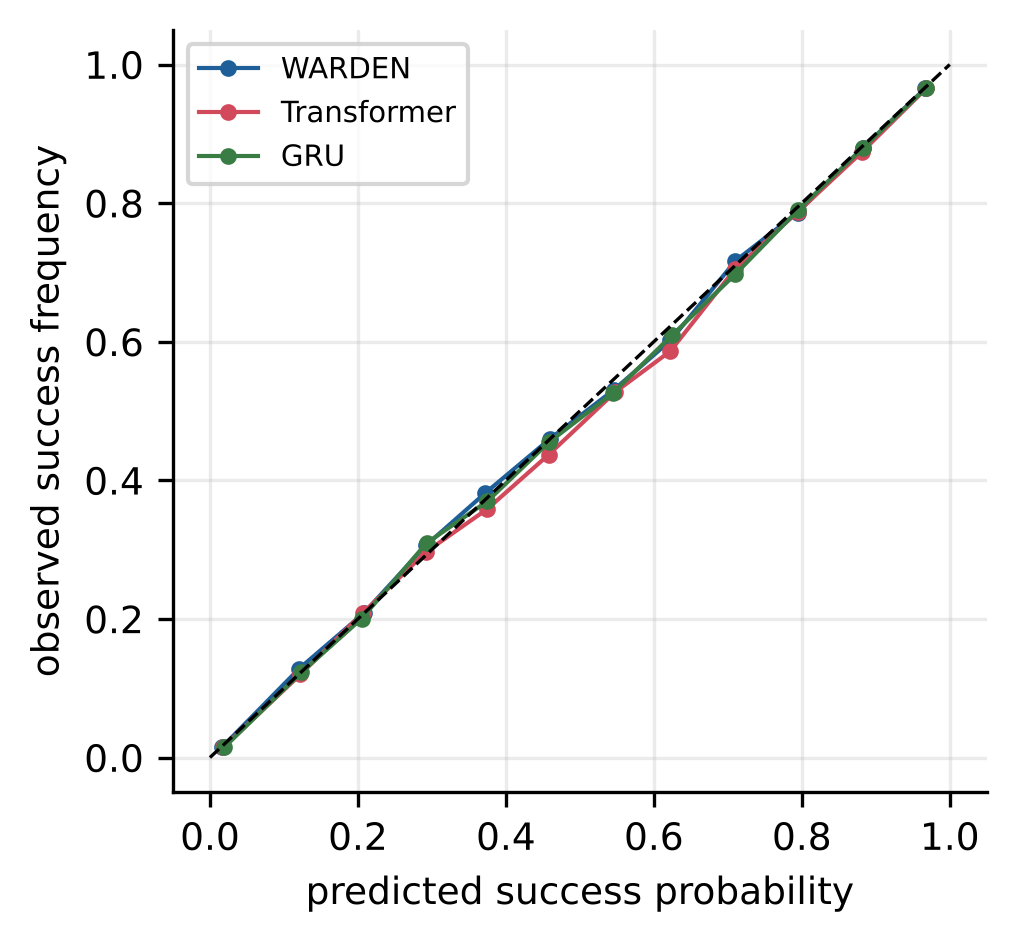
\includegraphics[width=0.5\textwidth,height=\textheight]{../figures/fig4_reliability.png}
\caption{\textbf{Fig. 4} Reliability diagram on the in-distribution test
split (all actions pooled, seed 1).}
\end{figure}

\hypertarget{risk-controlled-link-selection}{%
\subsection{6.3 Risk-controlled link
selection}\label{risk-controlled-link-selection}}

This subsection evaluates the base engine of Sections 4.1--4.3; the two
extensions are evaluated in Section 6.4.

Table 5 reports the decision metrics at \(\alpha=0.05\). The rule-based
policies never defer and therefore deliver readings with zero buffering
delay, but they fail often: the ADR-style rule with a 10 dB margin fails
15.8 \% of its attempts overall and 25.1 \% in rough water, and changing
the margin to 5 or 15 dB only moves the energy, not the risk. Naive
thresholds on the WARDEN-Net scores show the two classic failure modes
of uncertainty-unaware decisions: a threshold of 0.5 fails 16.7 \% of
the time, whereas the nominal threshold \(1-\alpha\) is so conservative
that more than half of the epochs are deferred and the delivery ratio
drops to 0.58.

The certified policies behave as designed. Mondrian LTT keeps the
realised risk at or below the target in every stratum, within the δ
allowance (largest stratum mean 0.051 ± 0.003), while global LTT
overshoots in rough water (0.053 ± 0.007) because its single threshold
is dominated by the calmer majority of the calibration data. Adding the
online update brings the risk to 0.050 in all three strata and every
seed. At this operating point WARDEN delivers 80.8 \% of all readings
with a mean latency of 13 min and spends 32.6 ± 2.2 mJ per delivered
reading, about five times less than the ADR rule (162.5 ± 9.8 mJ). It is
even lower than the 39.2 mJ of the oracle, which delivers almost every
reading and therefore also pays for the expensive frames needed in hard
conditions; the oracle still defers 11 \% of epochs to wait for a better
link. The price is a delivery ratio 3.4 points below the ADR rule,
because readings that cannot be sent reliably within 3 h are dropped.

\needspace{16\baselineskip}

\textbf{Table 5} Link-selection performance in distribution (α = 0.05, δ
= 0.1; mean of three seeds). ``Net'' is the WARDEN-Net ensemble; WARDEN
(full) adds the online update. Seed-to-seed standard deviations: overall
risk ≤ 0.024 (0.000 for WARDEN), RDR ≤ 0.037 (0.003 for WARDEN), energy
≤ 14.2 mJ (2.2 mJ for WARDEN).

\begin{longtable}[]{@{}
  >{\raggedright\arraybackslash}p{(\columnwidth - 16\tabcolsep) * \real{0.2500}}
  >{\raggedright\arraybackslash}p{(\columnwidth - 16\tabcolsep) * \real{0.0938}}
  >{\raggedright\arraybackslash}p{(\columnwidth - 16\tabcolsep) * \real{0.0938}}
  >{\raggedright\arraybackslash}p{(\columnwidth - 16\tabcolsep) * \real{0.0938}}
  >{\raggedright\arraybackslash}p{(\columnwidth - 16\tabcolsep) * \real{0.0938}}
  >{\raggedright\arraybackslash}p{(\columnwidth - 16\tabcolsep) * \real{0.0938}}
  >{\raggedright\arraybackslash}p{(\columnwidth - 16\tabcolsep) * \real{0.0938}}
  >{\raggedright\arraybackslash}p{(\columnwidth - 16\tabcolsep) * \real{0.0938}}
  >{\raggedright\arraybackslash}p{(\columnwidth - 16\tabcolsep) * \real{0.0938}}@{}}
\toprule\noalign{}
\begin{minipage}[b]{\linewidth}\raggedright
Policy
\end{minipage} & \begin{minipage}[b]{\linewidth}\raggedright
Risk
\end{minipage} & \begin{minipage}[b]{\linewidth}\raggedright
Calm
\end{minipage} & \begin{minipage}[b]{\linewidth}\raggedright
Mod.
\end{minipage} & \begin{minipage}[b]{\linewidth}\raggedright
Rough
\end{minipage} & \begin{minipage}[b]{\linewidth}\raggedright
Defer
\end{minipage} & \begin{minipage}[b]{\linewidth}\raggedright
RDR
\end{minipage} & \begin{minipage}[b]{\linewidth}\raggedright
Lat. (min)
\end{minipage} & \begin{minipage}[b]{\linewidth}\raggedright
E (mJ)
\end{minipage} \\
\midrule\noalign{}
\endhead
\bottomrule\noalign{}
\endlastfoot
ADR, 5 dB & 0.175 & 0.090 & 0.155 & 0.282 & 0 & 0.825 & 0 & 126.9 \\
ADR, 10 dB & 0.158 & 0.088 & 0.138 & 0.251 & 0 & \textbf{0.842} & 0 &
162.5 \\
ADR, 15 dB & 0.159 & 0.099 & 0.139 & 0.243 & 0 & 0.841 & 0 & 216.0 \\
Always SF12 & 0.172 & 0.114 & 0.154 & 0.255 & 0 & 0.828 & 0 & 239.1 \\
Satellite first & 0.202 & 0.152 & 0.185 & 0.271 & 0 & 0.798 & 0 &
396.8 \\
Net + thr. 0.5 & 0.167 & 0.118 & 0.154 & 0.225 & 0.103 & 0.779 & 3.8 &
54.3 \\
Net + thr. 1−α & 0.012 & 0.012 & 0.015 & 0.009 & 0.523 & 0.583 & 15.3 &
20.8 \\
Net + global LTT & 0.046 & 0.036 & 0.051 & 0.053 & 0.297 & 0.804 & 13.8
& 31.5 \\
Net + Mondrian LTT & 0.044 & 0.035 & 0.051 & 0.048 & 0.302 & 0.798 &
13.5 & 31.4 \\
\textbf{WARDEN (full)} & \textbf{0.050} & 0.050 & 0.050 & 0.050 & 0.293
& 0.808 & 13.3 & \textbf{32.6} \\
Oracle (bound) & 0 & 0 & 0 & 0 & 0.111 & 0.998 & 3.3 & 39.2 \\
\end{longtable}

Figure 5 shows the full trade-off as α varies from 0.01 to 0.20. Across
the whole range the certified policies use 3--8 times less energy per
delivered reading than the ADR family. The delivery ratio peaks near α =
0.10, where WARDEN delivers 82.6 ± 0.3 \% of readings at 41.3 ± 3.7 mJ,
i.e.~1.6 points below the 10 dB ADR rule for a quarter of its energy,
with a certified failure rate of 10 \% instead of an uncontrolled 15.8
\%. Beyond α = 0.10 the delivery ratio falls again, because each
additional failed unconfirmed frame destroys every buffered reading it
carries. When α is set to the risk that the ADR rule incurs on the
calibration days (0.166 ± 0.040), WARDEN matches that risk with 3.3
times less energy (48.6 versus 162.5 mJ) but a delivery ratio of 0.791
versus 0.842. The predictor matters only modestly at the policy level:
at α = 0.05, WARDEN-Net gives the lowest energy among all predictors
(32.6 mJ versus 33.8--38.8 mJ), whereas gradient boosting gives a
2.9-point higher delivery ratio at 17 \% more energy. Because the
certification layer is model agnostic, a deployment can choose either
operating point without losing the guarantee.

\begin{figure}
\centering
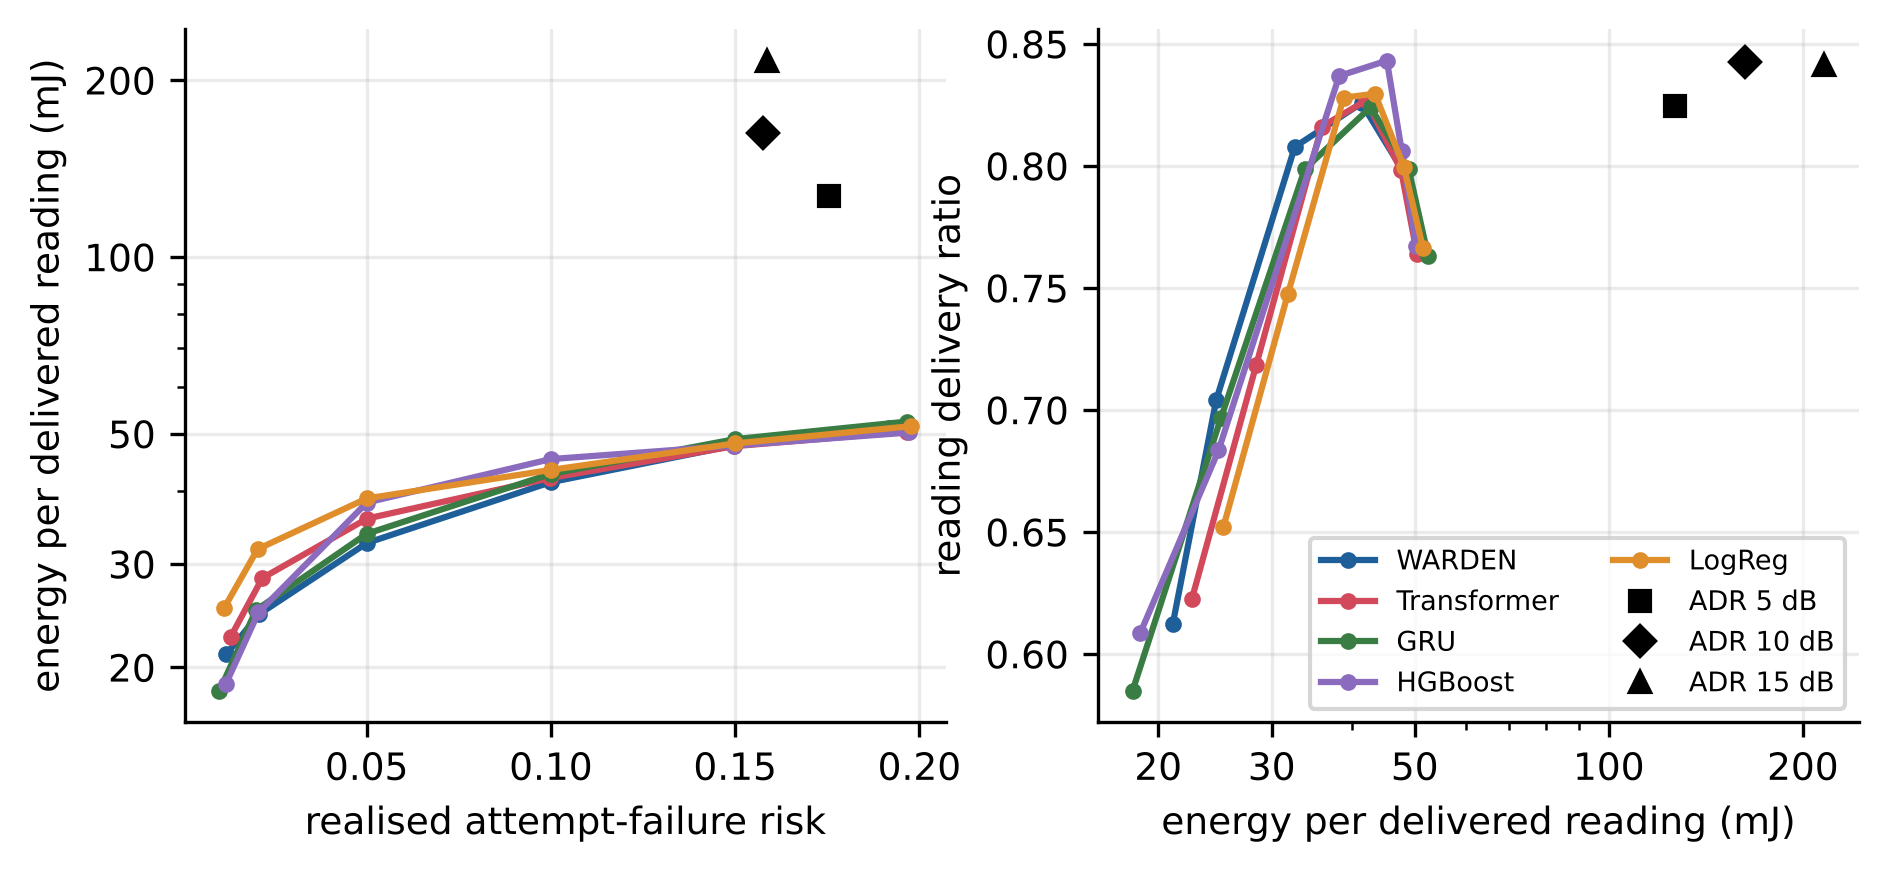
\includegraphics[width=1\textwidth,height=\textheight]{../figures/fig5_tradeoff.png}
\caption{\textbf{Fig. 5} Risk--energy and energy--delivery trade-offs
for \(\alpha \in \{0.01, 0.02, 0.05, 0.10, 0.15, 0.20\}\) with Mondrian
LTT and online update, compared with the ADR rule at 5, 10 and 15 dB
margins (in-distribution test, mean of three seeds).}
\end{figure}

\hypertarget{physics-informed-prior-and-urgency-aware-certification-warden-pi-u}{%
\subsection{6.4 Physics-informed prior and urgency-aware certification
(WARDEN-PI-U)}\label{physics-informed-prior-and-urgency-aware-certification-warden-pi-u}}

Table 6 and Fig. 6 compare the base engine with its two extensions under
the online certificate at α = 0.05. Every certified policy keeps the
realised attempt-failure risk at 0.049--0.050 in all three scenarios,
whereas the ADR rule fails 9.7--19.5 \% of its attempts. With the full
training set, the physics-residual head does not improve probabilistic
accuracy measurably (Brier 0.0842 versus 0.0839), because 36 days of
data already let the network learn most of the wave physics. It does,
however, improve the decisions: WARDEN-PI raises the reading delivery
ratio from 0.808 to 0.834 in distribution, from 0.788 to 0.813 under
storms and from 0.866 to 0.873 under the site shift, for 2--6 mJ more
energy per reading.

The urgency-aware cells give the largest gain. With
\(\alpha_U=\alpha=0.05\), so that no additional risk is accepted for
urgent traffic, WARDEN-PI-U delivers 86.2 ± 0.7 \% of all readings in
distribution, 84.5 ± 1.4 \% under severe storms and 90.0 ± 1.1 \% under
the site shift. This exceeds the delivery ratio of the 10 dB ADR rule in
distribution (84.2 \%) and under storms (80.5 \%) and matches it after
the site shift (90.3 \%), while using 4.2--4.6 times less energy per
reading and certifying a failure rate three to four times lower.
Ordinary traffic fails at exactly 5.0 \%; urgent epochs, about 6 \% of
all epochs, fail at only 3.3 \%, because their own working level adapts
to the conditions in which buffers approach expiry instead of inheriting
the threshold tuned for fresh data. The gain therefore comes from
allocating the same risk budget more intelligently, not from relaxing
it. The strongest learned baseline, gradient boosting, reaches 0.837 in
distribution at 38.2 mJ; giving it the physics prior as features does
not help (0.834), which indicates that the benefit of the prior is tied
to the residual design of (30) rather than to the extra inputs.

\needspace{16\baselineskip}

\textbf{Table 6} Certified link selection with the WARDEN extensions (α
= 0.05, α\_U = 0.05, online certificate; mean of three seeds,
delivery-ratio standard deviation in brackets)

\begin{longtable}[]{@{}
  >{\raggedright\arraybackslash}p{(\columnwidth - 14\tabcolsep) * \real{0.1064}}
  >{\raggedright\arraybackslash}p{(\columnwidth - 14\tabcolsep) * \real{0.2553}}
  >{\raggedright\arraybackslash}p{(\columnwidth - 14\tabcolsep) * \real{0.0957}}
  >{\raggedright\arraybackslash}p{(\columnwidth - 14\tabcolsep) * \real{0.0957}}
  >{\raggedright\arraybackslash}p{(\columnwidth - 14\tabcolsep) * \real{0.0957}}
  >{\raggedright\arraybackslash}p{(\columnwidth - 14\tabcolsep) * \real{0.1596}}
  >{\raggedright\arraybackslash}p{(\columnwidth - 14\tabcolsep) * \real{0.0957}}
  >{\raggedright\arraybackslash}p{(\columnwidth - 14\tabcolsep) * \real{0.0957}}@{}}
\toprule\noalign{}
\begin{minipage}[b]{\linewidth}\raggedright
Scenario
\end{minipage} & \begin{minipage}[b]{\linewidth}\raggedright
Policy
\end{minipage} & \begin{minipage}[b]{\linewidth}\raggedright
Risk
\end{minipage} & \begin{minipage}[b]{\linewidth}\raggedright
Ordinary
\end{minipage} & \begin{minipage}[b]{\linewidth}\raggedright
Urgent
\end{minipage} & \begin{minipage}[b]{\linewidth}\raggedright
RDR
\end{minipage} & \begin{minipage}[b]{\linewidth}\raggedright
Lat. (min)
\end{minipage} & \begin{minipage}[b]{\linewidth}\raggedright
E (mJ)
\end{minipage} \\
\midrule\noalign{}
\endhead
\bottomrule\noalign{}
\endlastfoot
ID & ADR, 10 dB & 0.158 & -- & -- & 0.842 (0.011) & 0 & 162.5 \\
ID & Gradient boosting & 0.050 & -- & -- & 0.837 (0.005) & 12.4 &
38.2 \\
ID & Boosting + prior & 0.050 & -- & -- & 0.834 (0.005) & 12.3 & 39.2 \\
ID & Physics prior only & 0.050 & -- & -- & 0.827 (0.008) & 16.3 &
37.8 \\
ID & WARDEN & 0.050 & -- & -- & 0.808 (0.003) & 13.3 & 32.6 \\
ID & WARDEN-PI & 0.050 & -- & -- & 0.834 (0.009) & 16.4 & 35.5 \\
ID & \textbf{WARDEN-PI-U} & \textbf{0.049} & 0.050 & 0.033 &
\textbf{0.862} (0.007) & 17.9 & 35.3 \\
OOD-A & ADR, 10 dB & 0.195 & -- & -- & 0.805 (0.021) & 0 & 185.9 \\
OOD-A & Gradient boosting & 0.050 & -- & -- & 0.812 (0.030) & 14.9 &
43.6 \\
OOD-A & WARDEN & 0.050 & -- & -- & 0.788 (0.028) & 16.8 & 35.6 \\
OOD-A & WARDEN-PI & 0.050 & -- & -- & 0.813 (0.028) & 18.7 & 41.1 \\
OOD-A & \textbf{WARDEN-PI-U} & \textbf{0.049} & 0.050 & 0.033 &
\textbf{0.845} (0.014) & 20.0 & 40.9 \\
OOD-B & ADR, 10 dB & 0.097 & -- & -- & 0.903 (0.003) & 0 & 111.2 \\
OOD-B & Gradient boosting & 0.050 & -- & -- & 0.875 (0.013) & 6.3 &
28.5 \\
OOD-B & WARDEN & 0.050 & -- & -- & 0.866 (0.008) & 7.6 & 25.5 \\
OOD-B & WARDEN-PI & 0.050 & -- & -- & 0.873 (0.015) & 9.6 & 26.6 \\
OOD-B & \textbf{WARDEN-PI-U} & \textbf{0.049} & 0.050 & 0.032 &
\textbf{0.900} (0.011) & 11.0 & 26.5 \\
\end{longtable}

\begin{figure}
\centering
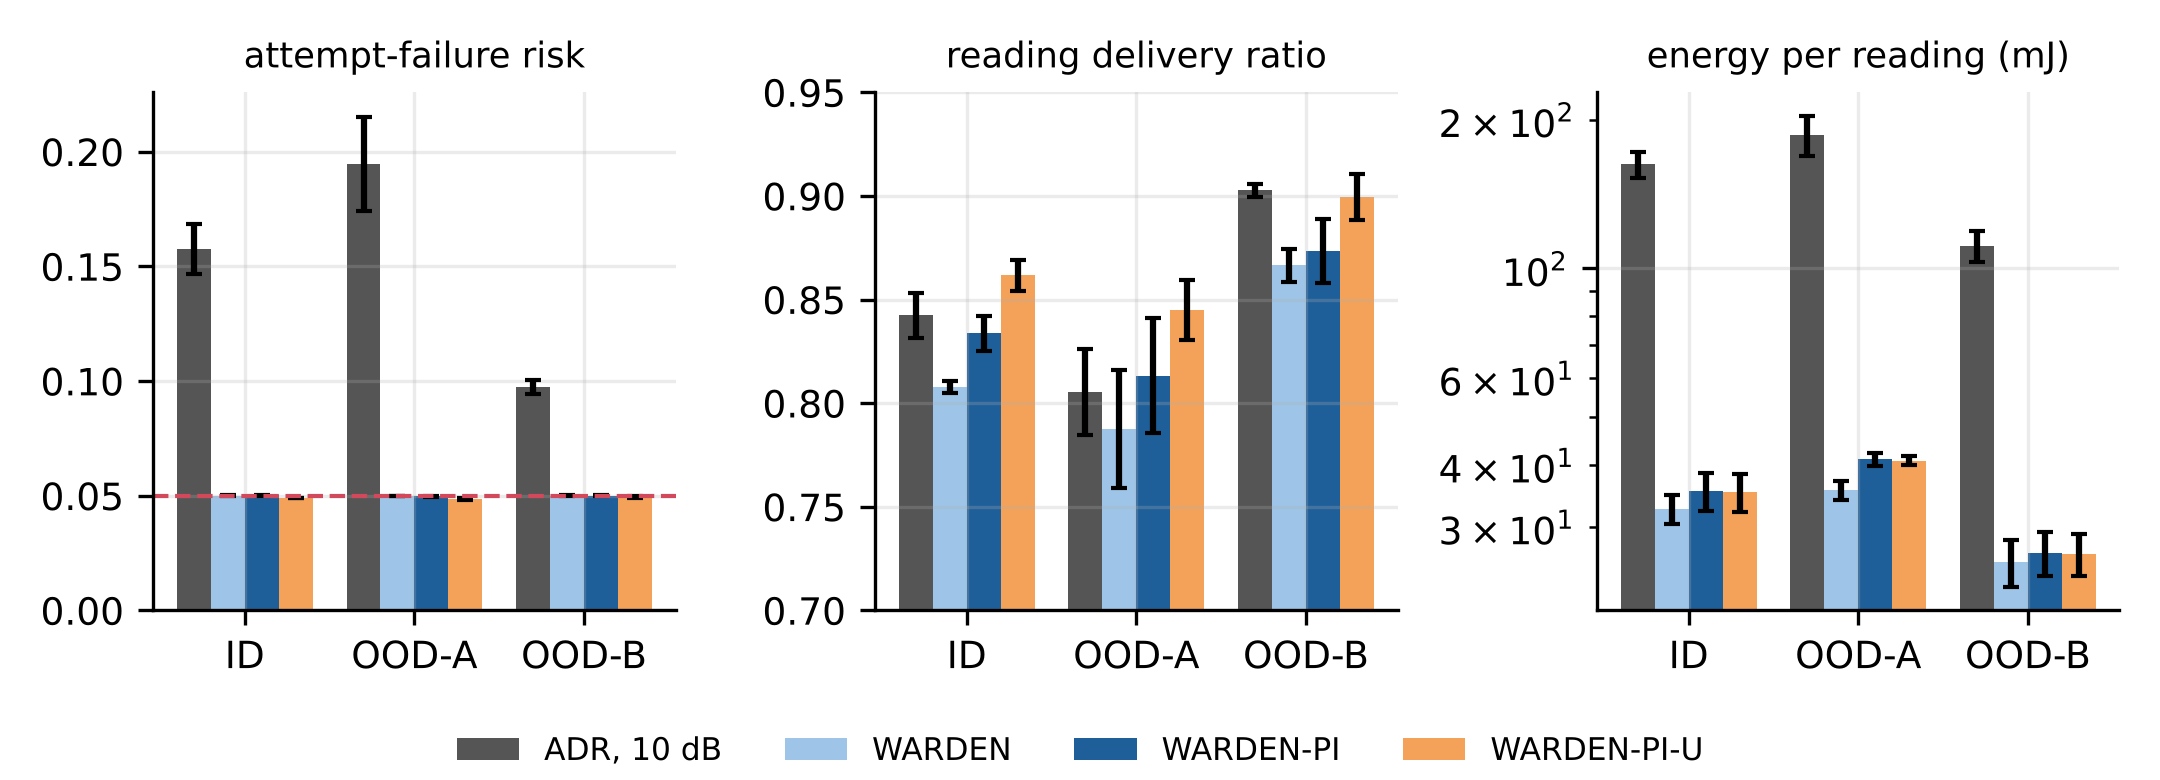
\includegraphics[width=1\textwidth,height=\textheight]{../figures/fig10_pi_u.png}
\caption{\textbf{Fig. 6} Attempt-failure risk, reading delivery ratio
and energy per reading of the ADR rule, WARDEN, WARDEN-PI and
WARDEN-PI-U in distribution and under the two shifts (α = α\_U = 0.05;
error bars: standard deviation over three seeds; energy on a logarithmic
axis).}
\end{figure}

\hypertarget{choosing-the-urgency-budget}{%
\subsection{6.5 Choosing the urgency
budget}\label{choosing-the-urgency-budget}}

Table 7 varies the urgent-traffic target. Raising \(\alpha_U\) above
\(\alpha\) is counter-productive: at \(\alpha_U=0.30\) the urgent cell
indeed fails 31 \% of the time, but each failed unconfirmed frame
destroys the whole buffer it carries, so the delivery ratio drops from
0.862 to 0.825. The best operating point is \(\alpha_U=\alpha\), which
is also the simplest to explain to an operator: one reliability target
for all traffic, applied separately to ordinary and urgent epochs. The
overall risk obeys the mixture (33) in every case.

\needspace{16\baselineskip}

\textbf{Table 7} Effect of the urgent-traffic target α\_U (in
distribution, α = 0.05; mean of three seeds)

\begin{longtable}[]{@{}lllllll@{}}
\toprule\noalign{}
α\_U & Risk (all) & Ordinary & Urgent & Urgent share & RDR & E (mJ) \\
\midrule\noalign{}
\endhead
\bottomrule\noalign{}
\endlastfoot
0.05 & 0.049 & 0.050 & 0.033 & 0.063 & \textbf{0.862} & 35.3 \\
0.10 & 0.051 & 0.050 & 0.077 & 0.042 & 0.858 & 36.1 \\
0.20 & 0.054 & 0.050 & 0.197 & 0.026 & 0.838 & 36.8 \\
0.30 & 0.055 & 0.050 & 0.311 & 0.020 & 0.825 & 37.0 \\
\end{longtable}

\hypertarget{data-efficiency-during-commissioning}{%
\subsection{6.6 Data efficiency during
commissioning}\label{data-efficiency-during-commissioning}}

A new buoy has little labelled data. Figure 7 repeats the experiment
with only 2, 4 or 8 days of training data (one further day for
temperature fitting and two days for calibration). Here the physics
prior pays off clearly. With two days of data, WARDEN-PI lowers the
Brier score of WARDEN-Net from 0.0958 to 0.0908 (5 \%) and raises the
delivery ratio from 0.746 to 0.773, and WARDEN-PI-U reaches 0.848 ±
0.011, above the ADR rule (0.842) and above gradient boosting (0.807)
and the physics prior alone (0.809), at 29 mJ instead of 162 mJ per
reading. With four and eight days, WARDEN-PI-U delivers 0.866 and 0.860.
The certified risk stays at 0.049--0.052 throughout, because the
guarantee does not depend on how good the predictor is; only the
efficiency does.

\begin{figure}
\centering
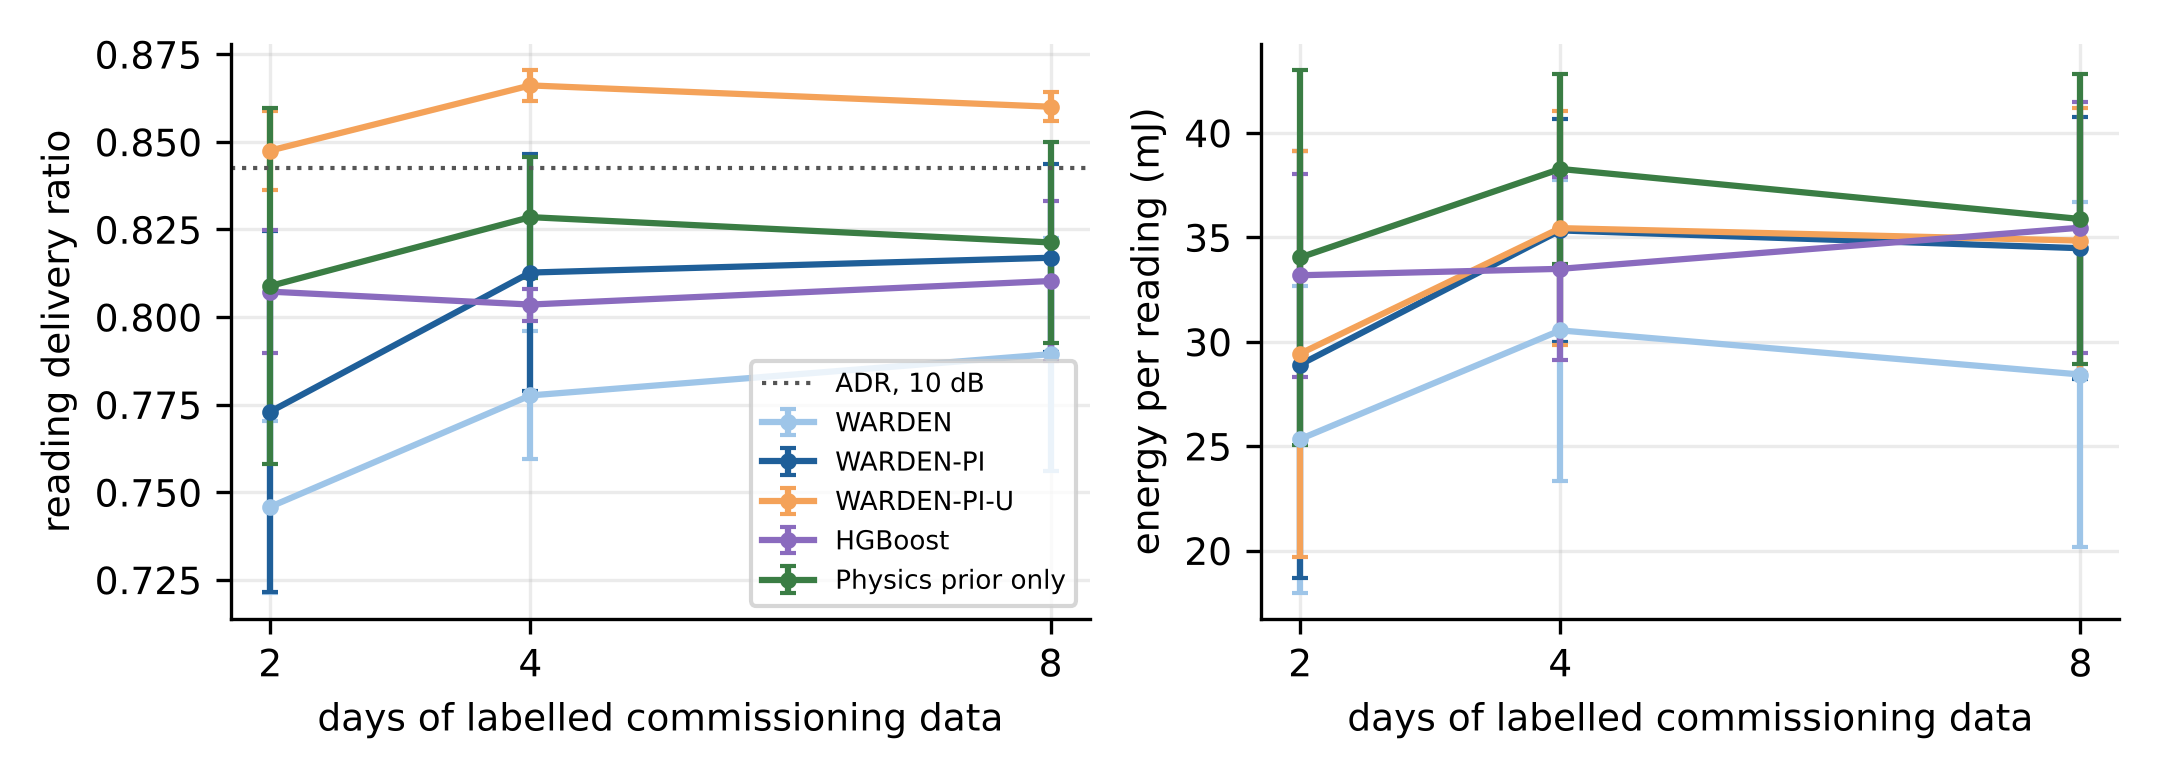
\includegraphics[width=1\textwidth,height=\textheight]{../figures/fig11_lowdata.png}
\caption{\textbf{Fig. 7} Commissioning with little data: reading
delivery ratio and energy per reading versus days of labelled training
data (α = 0.05; error bars: standard deviation over three seeds; dotted
line: ADR, 10 dB margin, trained on nothing).}
\end{figure}

\hypertarget{ablation-robustness-and-ood-analyses}{%
\section{7 Ablation, robustness and OOD
analyses}\label{ablation-robustness-and-ood-analyses}}

\hypertarget{out-of-distribution-deployments}{%
\subsection{7.1 Out-of-distribution
deployments}\label{out-of-distribution-deployments}}

Table 8 and Fig. 8 report the two shifted deployments with models and
thresholds taken unchanged from the in-distribution calibration. Under
severe storms (OOD-A) the ADR rule fails 19.5 \% of its attempts overall
and 26.6 \% in rough water. The offline certificate remains valid but
becomes conservative (risk 0.038), and the online update recovers the
unused risk budget, raising the delivery ratio from 0.743 to 0.788 at
the target risk of 0.050. The site and hardware shift (OOD-B) is harder
because it changes the conditional relationship between features and
outcomes. Here the offline certificate is violated for every predictor
that does not defer heavily: 0.052 for WARDEN-Net, 0.059--0.067 for the
other non-recurrent models, and 0.063 for WARDEN-Net without cross
attention. The online update restores 0.050 in every stratum within
about one day (Fig. 9), with a delivery ratio of 0.866 and 25.5 mJ per
reading, 4.4 times less than the ADR rule.

\needspace{16\baselineskip}

\textbf{Table 8} Behaviour under distribution shift (α = 0.05, mean of
three seeds; overall-risk standard deviation ≤ 0.021, 0.000 for WARDEN)

\begin{longtable}[]{@{}
  >{\raggedright\arraybackslash}p{(\columnwidth - 10\tabcolsep) * \real{0.1316}}
  >{\raggedright\arraybackslash}p{(\columnwidth - 10\tabcolsep) * \real{0.3947}}
  >{\raggedright\arraybackslash}p{(\columnwidth - 10\tabcolsep) * \real{0.1184}}
  >{\raggedright\arraybackslash}p{(\columnwidth - 10\tabcolsep) * \real{0.1184}}
  >{\raggedright\arraybackslash}p{(\columnwidth - 10\tabcolsep) * \real{0.1184}}
  >{\raggedright\arraybackslash}p{(\columnwidth - 10\tabcolsep) * \real{0.1184}}@{}}
\toprule\noalign{}
\begin{minipage}[b]{\linewidth}\raggedright
Scenario
\end{minipage} & \begin{minipage}[b]{\linewidth}\raggedright
Policy
\end{minipage} & \begin{minipage}[b]{\linewidth}\raggedright
Risk
\end{minipage} & \begin{minipage}[b]{\linewidth}\raggedright
Rough
\end{minipage} & \begin{minipage}[b]{\linewidth}\raggedright
RDR
\end{minipage} & \begin{minipage}[b]{\linewidth}\raggedright
E (mJ)
\end{minipage} \\
\midrule\noalign{}
\endhead
\bottomrule\noalign{}
\endlastfoot
A storms & ADR, 10 dB & 0.195 & 0.266 & 0.805 & 185.9 \\
A storms & Net + Mondrian LTT & 0.038 & 0.037 & 0.743 & 32.9 \\
A storms & \textbf{WARDEN (full)} & \textbf{0.050} & 0.050 & 0.788 &
35.6 \\
B site & ADR, 10 dB & 0.097 & 0.165 & 0.903 & 111.2 \\
B site & Transformer + Mondrian LTT & 0.063 & 0.063 & 0.887 & 30.8 \\
B site & Boosting + Mondrian LTT & 0.059 & 0.051 & 0.887 & 30.9 \\
B site & Net + global LTT & 0.053 & 0.061 & 0.871 & 27.2 \\
B site & Net + Mondrian LTT & 0.052 & 0.055 & 0.869 & 26.7 \\
B site & \textbf{WARDEN (full)} & \textbf{0.050} & 0.050 & 0.866 &
\textbf{25.5} \\
\end{longtable}

\begin{figure}
\centering
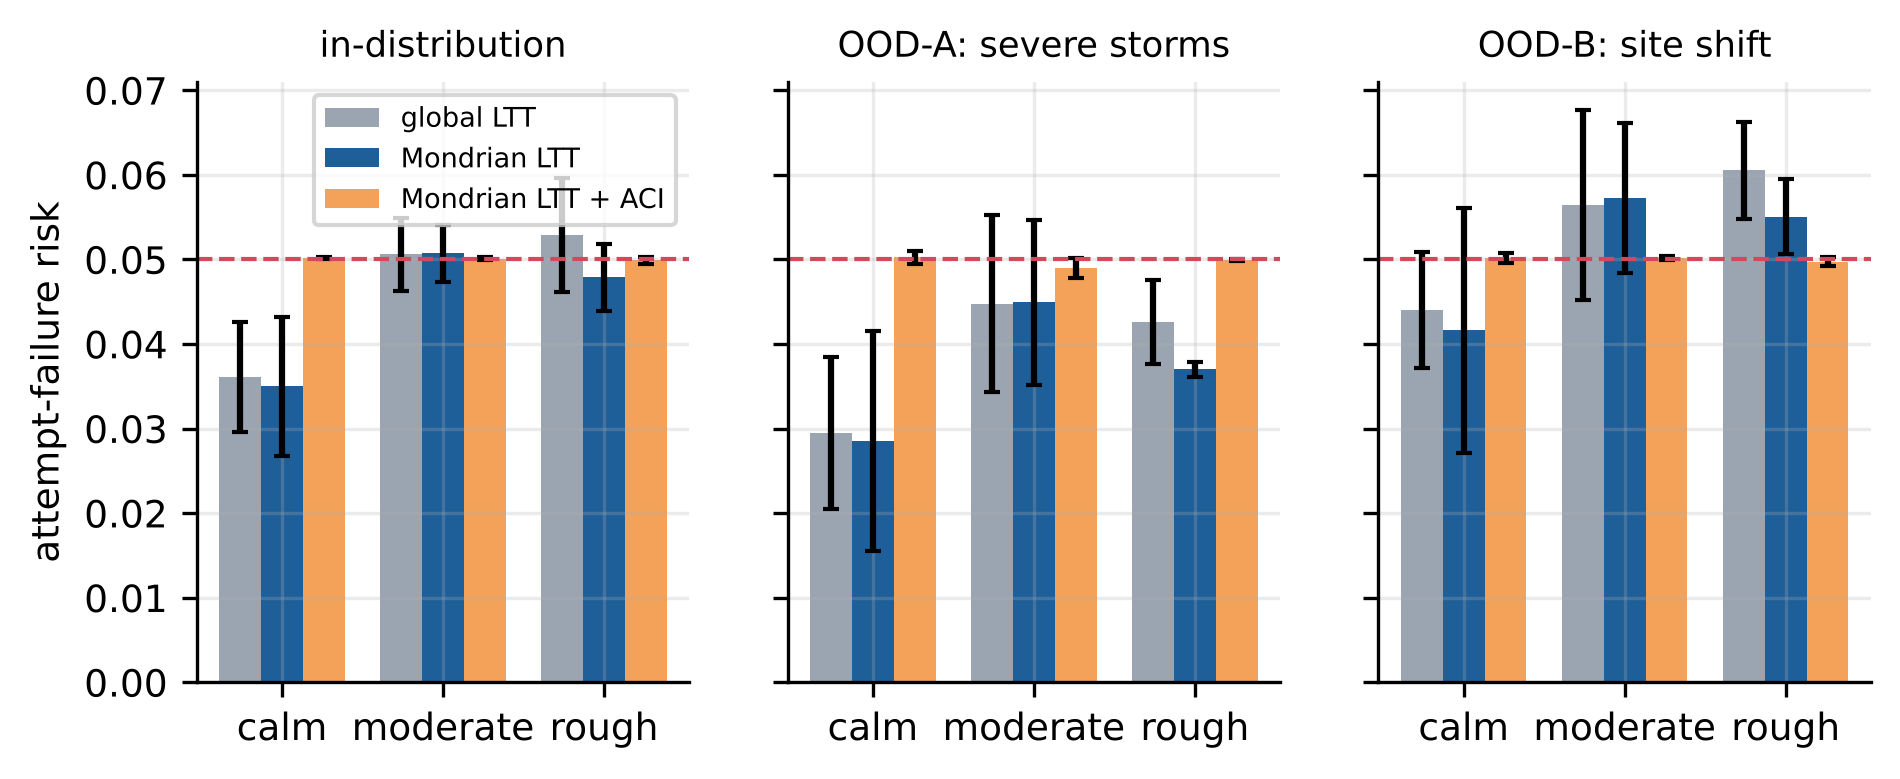
\includegraphics[width=1\textwidth,height=\textheight]{../figures/fig6_stratum_risk.png}
\caption{\textbf{Fig. 8} Per-stratum attempt-failure risk of global LTT,
Mondrian LTT and Mondrian LTT with online update in distribution and
under the two shifts (error bars: std over three seeds; dashed line:
α).}
\end{figure}

\begin{figure}
\centering
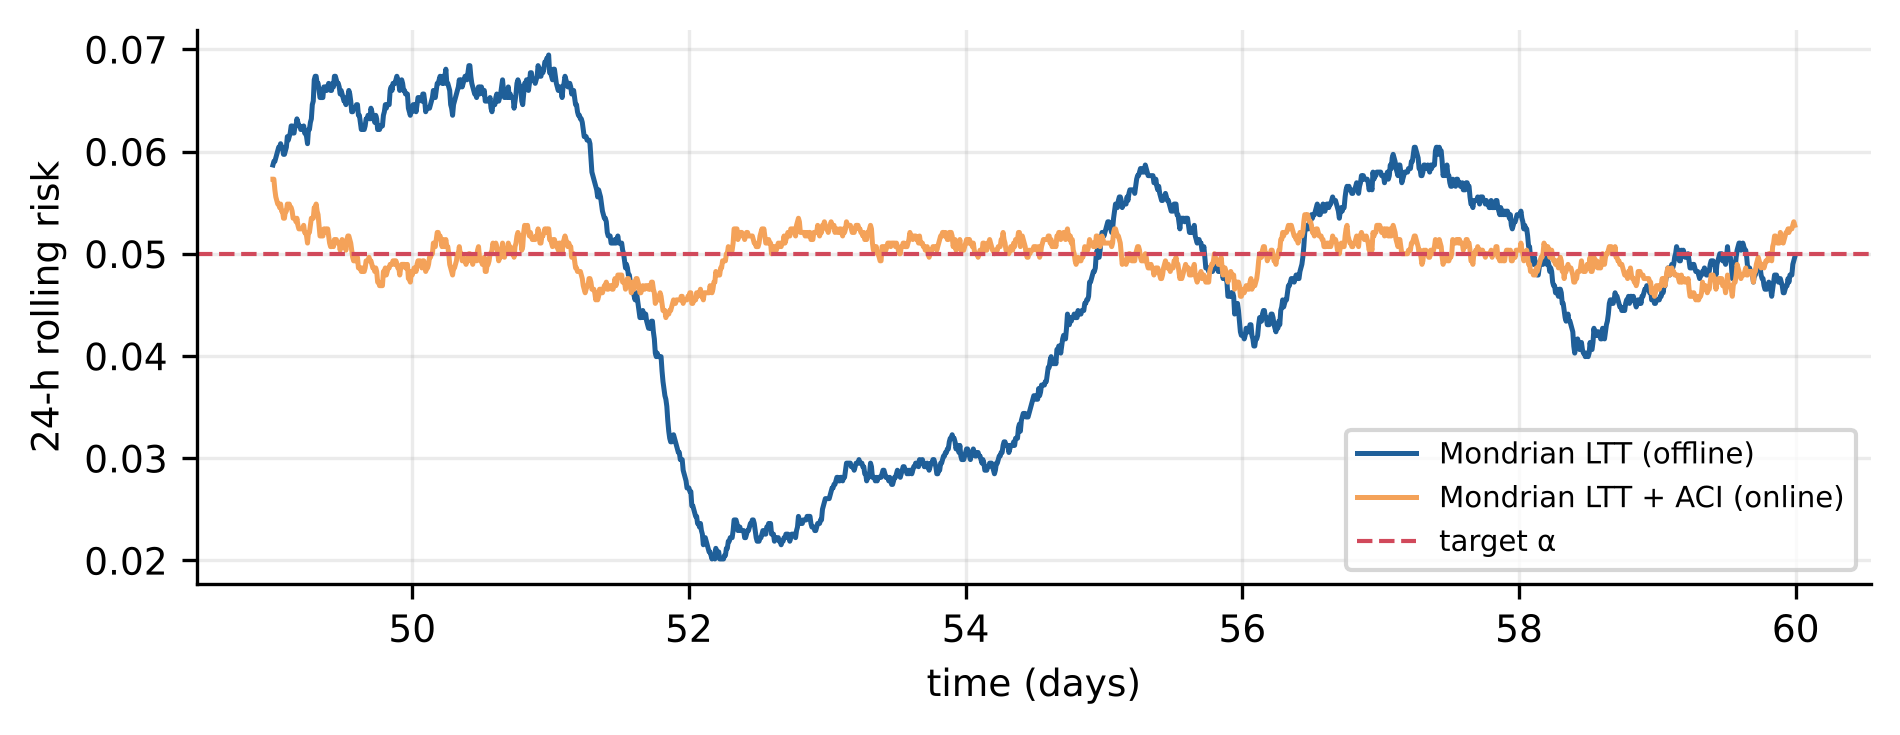
\includegraphics[width=0.95\textwidth,height=\textheight]{../figures/fig7_online_site_shift.png}
\caption{\textbf{Fig. 9} 24-h rolling risk under the site shift (OOD-B,
seed 1). The offline certificate drifts between 2 \% and 7 \%, while the
online update holds the risk near α.}
\end{figure}

\hypertarget{ablation-of-warden-components}{%
\subsection{7.2 Ablation of WARDEN
components}\label{ablation-of-warden-components}}

Table 9 isolates each component under offline Mondrian LTT, where
differences in score quality show up directly as deferral and delivery.
Removing the IMU features or setting the uncertainty penalty to κ = 0
makes the policy much more conservative and less stable across seeds
(deferral 0.39 ± 0.09 and 0.38 ± 0.11 instead of 0.30 ± 0.01; delivery
0.75 instead of 0.80). Inspection shows the mechanism: without sea-state
information or ensemble spread, the empirical risk curve of the calm
stratum is ragged, and fixed-sequence testing stops at a high threshold.
Removing cross attention barely changes in-distribution behaviour but
raises the risk under the site shift from 0.052 to 0.063, and removing
the SF-monotone head increases energy per reading by 9 \% (34.2 versus
31.4 mJ) and raises the OOD-B risk to 0.056. A single network instead of
a three-member ensemble costs 5 \% more energy.

\needspace{16\baselineskip}

\textbf{Table 9} Ablation with offline Mondrian LTT (α = 0.05; ID: in
distribution; B: OOD-B site shift; mean of three seeds, deferral with
standard deviation)

\begin{longtable}[]{@{}
  >{\raggedright\arraybackslash}p{(\columnwidth - 10\tabcolsep) * \real{0.3200}}
  >{\raggedright\arraybackslash}p{(\columnwidth - 10\tabcolsep) * \real{0.2000}}
  >{\raggedright\arraybackslash}p{(\columnwidth - 10\tabcolsep) * \real{0.1200}}
  >{\raggedright\arraybackslash}p{(\columnwidth - 10\tabcolsep) * \real{0.1200}}
  >{\raggedright\arraybackslash}p{(\columnwidth - 10\tabcolsep) * \real{0.1200}}
  >{\raggedright\arraybackslash}p{(\columnwidth - 10\tabcolsep) * \real{0.1200}}@{}}
\toprule\noalign{}
\begin{minipage}[b]{\linewidth}\raggedright
Variant
\end{minipage} & \begin{minipage}[b]{\linewidth}\raggedright
Defer (ID)
\end{minipage} & \begin{minipage}[b]{\linewidth}\raggedright
RDR (ID)
\end{minipage} & \begin{minipage}[b]{\linewidth}\raggedright
E (ID, mJ)
\end{minipage} & \begin{minipage}[b]{\linewidth}\raggedright
Risk (B)
\end{minipage} & \begin{minipage}[b]{\linewidth}\raggedright
ECE (B)
\end{minipage} \\
\midrule\noalign{}
\endhead
\bottomrule\noalign{}
\endlastfoot
WARDEN-Net, full & 0.302 ± 0.006 & 0.798 & 31.4 & 0.052 & 0.0229 \\
without IMU features & 0.390 ± 0.088 & 0.748 & 28.5 & 0.055 & 0.0228 \\
without cross attention & 0.305 ± 0.004 & 0.807 & 32.8 & 0.063 &
0.0376 \\
without SF-monotone head & 0.292 ± 0.012 & 0.797 & 34.2 & 0.056 &
0.0267 \\
single network (M = 1) & 0.302 ± 0.004 & 0.799 & 33.0 & 0.054 &
0.0258 \\
no penalty (κ = 0) & 0.377 ± 0.105 & 0.752 & 30.4 & -- & -- \\
\end{longtable}

Figure 10 visualises the cross-attention weights learned by WARDEN-Net.
In calm water the query concentrates on the most recent beacons, which
carry the slowly varying shadowing and ducting state; in rough water the
weights flatten and older steps receive more mass, consistent with
averaging out wave-induced fluctuations. This behaviour was not imposed
and supports the design rationale of Section 4.2.

\begin{figure}
\centering
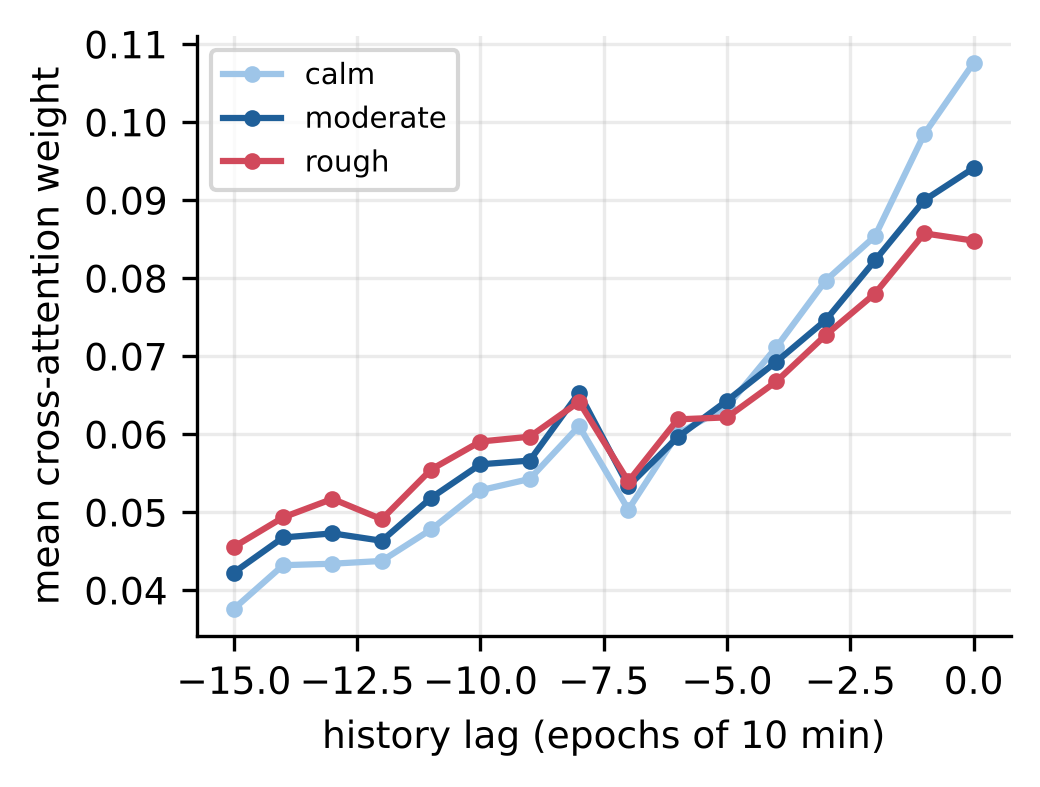
\includegraphics[width=0.5\textwidth,height=\textheight]{../figures/fig9_attention.png}
\caption{\textbf{Fig. 10} Mean cross-attention weight over history lag,
by IMU sea-state stratum (seed 1, 2 000 test windows).}
\end{figure}

\hypertarget{robustness-and-calibration-set-size}{%
\subsection{7.3 Robustness and calibration-set
size}\label{robustness-and-calibration-set-size}}

With IMU noise raised from 8 \% to 30 \%, offline Mondrian LTT still
meets the target (0.042 ± 0.004) and the online version holds 0.050 with
a delivery ratio of 0.815. With beacon SNR noise raised from 1 dB to 3
dB, the offline certificate sits at the boundary (0.050 ± 0.007,
moderate stratum 0.055), and the online update again restores 0.050 in
all strata. The ADR rule is unaffected by IMU noise but keeps its 15.8
\% risk.

Figure 11 shows the effect of the calibration-set size. With only 250
calibration epochs, which corresponds to less than two days of a single
buoy, 3.3 \% of the 60 random draws violated the target, below the
permitted δ = 10 \%, and the worst draw reached 0.053. From 500 epochs
upwards no draw violated the target. Larger calibration sets reduce
conservatism: the deferral rate falls from 0.47 at n = 250 to 0.31 at n
= 4 000.

\begin{figure}
\centering
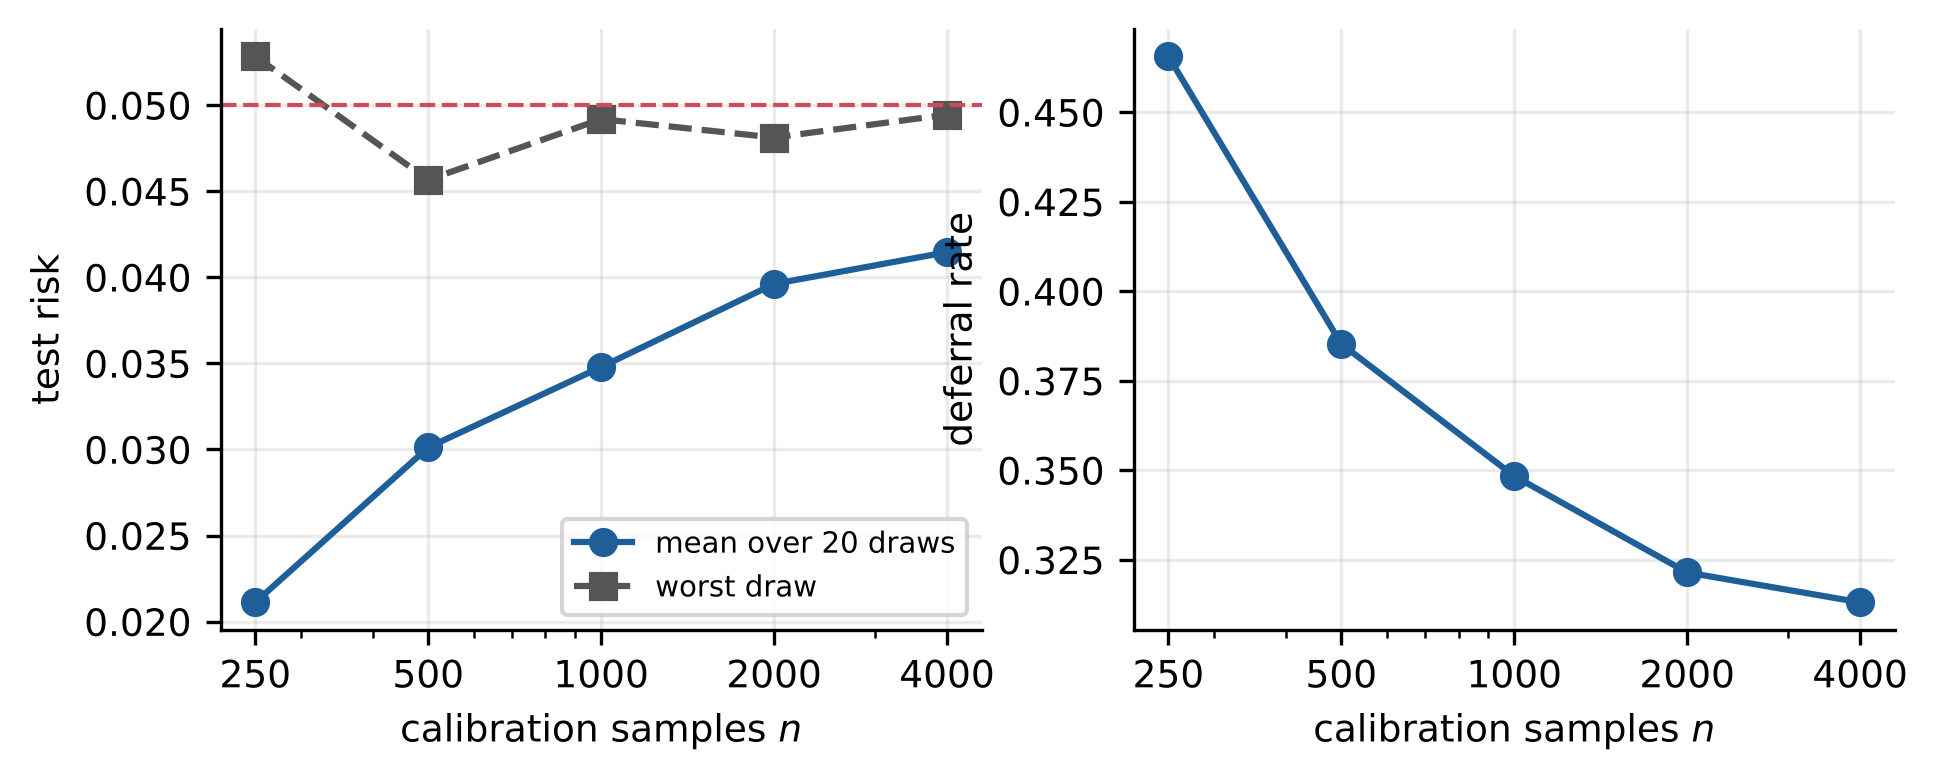
\includegraphics[width=0.95\textwidth,height=\textheight]{../figures/fig8_calibration_size.png}
\caption{\textbf{Fig. 11} Calibration-set size: test risk (mean and
worst of 20 random draws per seed) and deferral rate.}
\end{figure}

\hypertarget{robustness-to-a-misspecified-physics-prior}{%
\subsection{7.4 Robustness to a misspecified physics
prior}\label{robustness-to-a-misspecified-physics-prior}}

A physics prior is only as good as its model. Table 10 trains and
calibrates WARDEN-PI with the deliberately biased prior of Section 5.2.
In distribution the residual network absorbs most of the error: the
delivery ratio is unchanged (0.837 versus 0.834) and energy rises by 12
\%. Under the two shifts the wrong prior becomes visibly miscalibrated
(ECE 0.19--0.21 instead of 0.014--0.022), the policy compensates by
choosing more robust and more expensive actions, and energy per reading
roughly doubles. The certificate, however, still holds: the realised
risk is 0.045--0.050 in every scenario. A wrong physics model therefore
costs energy but not reliability, which is the property a
safety-critical ocean deployment needs.

\needspace{16\baselineskip}

\textbf{Table 10} WARDEN-PI with correct and misspecified physics prior
(α = 0.05, online certificate; mean of three seeds)

\begin{longtable}[]{@{}llllll@{}}
\toprule\noalign{}
Scenario & Prior & Risk & RDR & E (mJ) & ECE \\
\midrule\noalign{}
\endhead
\bottomrule\noalign{}
\endlastfoot
ID & correct & 0.050 & 0.834 & 35.5 & 0.008 \\
ID & misspecified & 0.050 & 0.837 & 39.7 & 0.016 \\
OOD-A & correct & 0.050 & 0.813 & 41.1 & 0.014 \\
OOD-A & misspecified & 0.045 & 0.857 & 73.6 & 0.213 \\
OOD-B & correct & 0.050 & 0.873 & 26.6 & 0.022 \\
OOD-B & misspecified & 0.048 & 0.897 & 51.9 & 0.194 \\
\end{longtable}

\hypertarget{discussion-utility-and-limitations}{%
\section{8 Discussion, utility and
limitations}\label{discussion-utility-and-limitations}}

WARDEN turns link reliability into a design parameter. The operator sets
one failure target α and obtains it, per sea state, on every buoy;
WARDEN-PI-U then delivers at least as many readings as an ADR-style rule
in calm and stormy seas while spending four to five times less energy,
which for a battery-limited buoy translates almost directly into service
lifetime. The physics prior makes the scheme usable from the first days
of a deployment, and the urgency cells remove the usual penalty of
cautious policies, namely data that expire in the buffer. No change to
LoRaWAN or LR-FHSS radios is needed: only a beacon with a receipt
bitmap, a tide table and a small on-board model.

The limitations are equally concrete. All results come from a synthetic,
physics-guided test bed, and the physics prior uses the same family of
propagation models as the simulator; Table 10 bounds the damage of a
wrong model, but sea trials are required before claims about real
deployments. Training labels for all actions require probe frames in
practice. Ordinary deliveries are delayed by about 15 min on average,
and the online guarantee is a long-run average that does not bound short
bursts of failures.

\hypertarget{conclusion}{%
\section{9 Conclusion}\label{conclusion}}

This paper presented WARDEN, a wave aware decision engine that lets an
ocean monitoring buoy choose between LoRa spreading factors, a
direct-to-satellite LR-FHSS frame and buffering with a certified bound
on attempt failures. WARDEN combines four elements that had not been
brought together for maritime links: a closed-form, wave-integrated
physics prior driven by the buoy's own IMU; an attention network with
sea-state-conditioned cross attention, an SF-monotone head and a
physics-residual output; Mondrian Learn-then-Test calibration per sea
state; and adaptive conformal updates organised in urgency-aware cells.
In a 60-day, 20-buoy test bed with storm and site shifts, the full
system held the failure rate at the 5 \% target in every sea state and
scenario, delivered 84.5--90.0 \% of all readings, matching or exceeding
an ADR-style rule that failed 10--20 \% of its attempts, and used
4.2--4.6 times less energy per reading. The certificate held even with a
deliberately wrong physics model, and two days of commissioning data
sufficed to outperform the rule-based baseline. Future work will
validate WARDEN in sea trials, replace full-label training with bandit
feedback, bound short-term failure bursts, and extend the action set to
multi-gateway and NB-IoT non-terrestrial links.

\hypertarget{declarations}{%
\section{Declarations}\label{declarations}}

\textbf{Funding} This research received no specific grant from any funding agency in the public, commercial or not-for-profit sectors.

\textbf{Competing interests} The authors declare no competing interests.

\textbf{Data availability} All data are generated by the released
simulator; the scripts reproduce every table and figure.

\textbf{Code availability} Source code is available at
https://github.com/iitrky/warden.

\textbf{Author contributions} To be completed according to the CRediT
taxonomy.

\hypertarget{references}{%
\section{References}\label{references}}

\begin{enumerate}
\def\labelenumi{\arabic{enumi}.}
\tightlist
\item
  Xia T, Wang MM, Zhang J, Wang L (2020) Maritime Internet of Things:
  Challenges and solutions. IEEE Wirel Commun 27(2):188--196.
  \url{https://doi.org/10.1109/MWC.001.1900322}
\item
  Alqurashi FS, Trichili A, Saeed N, Ooi BS, Alouini M-S (2023) Maritime
  communications: A survey on enabling technologies, opportunities, and
  challenges. IEEE Internet Things J 10(4):3525--3547.
  \url{https://doi.org/10.1109/JIOT.2022.3219674}
\item
  Wei T, Feng W, Chen Y, Wang C-X, Ge N, Lu J (2021) Hybrid
  satellite-terrestrial communication networks for the maritime Internet
  of Things: Key technologies, opportunities, and challenges. IEEE
  Internet Things J 8(11):8910--8934.
  \url{https://doi.org/10.1109/JIOT.2021.3056091}
\item
  Jahanbakht M, Xiang W, Hanzo L, Rahimi Azghadi M (2021) Internet of
  underwater things and big marine data analytics: A comprehensive
  survey. IEEE Commun Surv Tutor 23(2):904--956.
  \url{https://doi.org/10.1109/COMST.2021.3053118}
\item
  Parri L, Parrino S, Peruzzi G, Pozzebon A (2021) Offshore LoRaWAN
  networking: Transmission performances analysis under different
  environmental conditions. IEEE Trans Instrum Meas 70:1--10.
  \url{https://doi.org/10.1109/TIM.2020.3031193}
\item
  Centenaro M, Costa CE, Granelli F, Sacchi C, Vangelista L (2021) A
  survey on technologies, standards and open challenges in satellite
  IoT. IEEE Commun Surv Tutor 23(3):1693--1720.
  \url{https://doi.org/10.1109/COMST.2021.3078433}
\item
  Kodheli O, Lagunas E, Maturo N, Sharma SK, Shankar B, Montoya JFM,
  Duncan JCM, Spano D, Chatzinotas S, Kisseleff S, Querol J, Lei L, Vu
  TX, Goussetis G (2021) Satellite communications in the new space era:
  A survey and future challenges. IEEE Commun Surv Tutor 23(1):70--109.
  \url{https://doi.org/10.1109/COMST.2020.3028247}
\item
  Huo Y, Dong X, Beatty S (2020) Cellular communications in ocean waves
  for maritime Internet of Things. IEEE Internet Things J
  7(10):9965--9979. \url{https://doi.org/10.1109/JIOT.2020.2988634}
\item
  He Y, Wang C-X, Chang H, Huang J, Sun J, Zhang W, Aggoune E-HM (2022)
  A novel 3D non-stationary maritime wireless channel model. IEEE Trans
  Commun 70(3):2102. \url{https://doi.org/10.1109/TCOMM.2021.3134275}
\item
  Liu Y, Wang C-X, Chang H, He Y, Bian J (2021) A novel non-stationary
  6G UAV channel model for maritime communications. IEEE J Sel Areas
  Commun 39(10):2992--3005.
  \url{https://doi.org/10.1109/JSAC.2021.3088664}
\item
  Zhang H, Zhou T, Xu T, et al (2022) Statistical modeling of
  evaporation duct channel for maritime broadband communications. IEEE
  Trans Veh Technol 71(10):10228.
  \url{https://doi.org/10.1109/TVT.2022.3187753}
\item
  Robinson L, Newe T, Burke J, Toal D (2022) A simulated and
  experimental analysis of evaporation duct effects on microwave
  communications in the Irish Sea. IEEE Trans Antennas Propag 70(6).
  \url{https://doi.org/10.1109/TAP.2022.3145460}
\item
  Fang X, Feng W, Wang Y, Chen Y, Ge N, Ding Z, Zhu H (2023) NOMA-based
  hybrid satellite-UAV-terrestrial networks for 6G maritime coverage.
  IEEE Trans Wirel Commun 22(1):138--152.
  \url{https://doi.org/10.1109/TWC.2022.3191719}
\item
  Li X, Feng W, Wang J, Chen Y, Ge N, Wang C-X (2020) Enabling 5G on the
  ocean: A hybrid satellite-UAV-terrestrial network solution. IEEE Wirel
  Commun 27(6):116--121. \url{https://doi.org/10.1109/MWC.001.2000076}
\item
  Boquet G, Tuset-Peiró P, Adelantado F, Watteyne T, Vilajosana X (2021)
  LR-FHSS: Overview and performance analysis. IEEE Commun Mag
  59(3):30--36. \url{https://doi.org/10.1109/MCOM.001.2000627}
\item
  Ullah MA, Mikhaylov K, Alves H (2022) Analysis and simulation of
  LoRaWAN LR-FHSS for direct-to-satellite scenario. IEEE Wirel Commun
  Lett 11(3):548--552. \url{https://doi.org/10.1109/LWC.2021.3135984}
\item
  Ullah MA, Pasolini G, Mikhaylov K, Alves H (2023) Understanding the
  limits of LoRa direct-to-satellite: The Doppler perspectives. IEEE
  Open J Commun Soc. \url{https://doi.org/10.1109/OJCOMS.2023.3337004}
\item
  Alvarez G, Fraire JA, Hassan KA, Céspedes S, Pesch D (2022) Uplink
  transmission policies for LoRa-based direct-to-satellite IoT. IEEE
  Access 10:72687--72701.
  \url{https://doi.org/10.1109/ACCESS.2022.3189647}
\item
  Røste T, Yang K, Wen C (2023) Satellite to buoy IoT communications in
  the Arctic Ocean. Front Mar Sci 10:1153798.
  \url{https://doi.org/10.3389/fmars.2023.1153798}
\item
  Zhou T, Liu X, Xiang Z, Zhang H, Ai B, Liu L, Jing X (2024)
  Transformer network based channel prediction for CSI feedback
  enhancement in AI-native air interface. IEEE Trans Wirel Commun.
  \url{https://doi.org/10.1109/TWC.2024.3379123}
\item
  Rizzello V, Böck B, Joham M, Utschick W (2024) Reverse ordering
  techniques for attention-based channel prediction. IEEE Open J Signal
  Process. \url{https://doi.org/10.1109/OJSP.2023.3344024}
\item
  Lim B, Arık SÖ, Loeff N, Pfister T (2021) Temporal fusion transformers
  for interpretable multi-horizon time series forecasting. Int J
  Forecast 37(4):1748--1764.
  \url{https://doi.org/10.1016/j.ijforecast.2021.03.012}
\item
  Strzoda A, Grochla K, Głomb P, Madej A (2023) Link failure prediction
  in LoRa networks. In: Proc Int Wirel Commun Mob Comput Conf (IWCMC).
  IEEE. \url{https://doi.org/10.1109/IWCMC58020.2023.10183185}
\item
  Shilpa B, Gupta HP, Jha RK, Hashmi SS (2024) LoRa interference issues
  and solution approaches in dense IoT networks: A review. Telecommun
  Syst 87:517--539. \url{https://doi.org/10.1007/s11235-024-01192-9}
\item
  Lyimo M, Mgawe B, Leo J, Dida M, Michael K (2026) LSTM-based deep
  reinforcement learning for ISI mitigation in maritime LoRaWAN. Phys
  Commun 75:103063. \url{https://doi.org/10.1016/j.phycom.2026.103063}
\item
  Leonardi L, Iannizzotto G, Pirri M, Patti G, Pirri A, Lo Bello L
  (2025) A deep learning-based adaptive data rate algorithm for LoRaWAN
  networks. Internet Things 101786.
  \url{https://doi.org/10.1016/j.iot.2025.101786}
\item
  Nisar F, Amin M, Irshad MT, Hadi HJ, Ahmad N, Ladan M (2025) Machine
  learning-based spreading factor optimization in LoRaWAN networks.
  Front Comput Sci 7:1666262.
  \url{https://doi.org/10.3389/fcomp.2025.1666262}
\item
  Dargie W, Poellabauer C, Tasissa A (2025) Prediction of the power of
  low-power networks using inertial sensors. IEEE Trans Instrum Meas
  74:5506410
\item
  Cohen KM, Park S, Simeone O, Shamai S (2023) Calibrating AI models for
  wireless communications via conformal prediction. IEEE Trans Mach
  Learn Commun Netw 1:296--312.
  \url{https://doi.org/10.1109/TMLCN.2023.3319282}
\item
  Angelopoulos AN, Bates S (2023) Conformal prediction: A gentle
  introduction. Found Trends Mach Learn 16(4):494--591.
  \url{https://doi.org/10.1561/2200000101}
\item
  Deng W, Shi B, Li M, Simeone O (2026) SCAN-BEST: Sub-6GHz-aided
  near-field beam selection with formal reliability guarantees. IEEE
  Trans Cogn Commun Netw.
  \url{https://doi.org/10.1109/TCCN.2026.3657091}
\item
  Bates S, Angelopoulos A, Lei L, Malik J, Jordan MI (2021)
  Distribution-free, risk-controlling prediction sets. J ACM 68(6):43.
  \url{https://doi.org/10.1145/3478535}
\item
  Angelopoulos AN, Bates S, Fisch A, Lei L, Schuster T (2024) Conformal
  risk control. In: Proc Int Conf Learn Represent (ICLR).
  \url{https://proceedings.iclr.cc/paper_files/paper/2024/hash/f3549ef9b5ff520a7e41ff3cc306ab2b-Abstract-Conference.html}
\item
  Angelopoulos AN, Bates S, Candès EJ, Jordan MI, Lei L (2025) Learn
  then test: Calibrating predictive algorithms to achieve risk control.
  Ann Appl Stat 19:1641--1662. \url{https://doi.org/10.1214/24-AOAS1998}
\item
  Gibbs I, Candès E (2021) Adaptive conformal inference under
  distribution shift. In: Adv Neural Inf Process Syst 34 (NeurIPS).
  \url{https://proceedings.neurips.cc/paper/2021/hash/0d441de75945e5acbc865406fc9a2559-Abstract.html}
\item
  Parri L, Parrino S, Peruzzi G, Pozzebon A (2019) Low power wide area
  networks (LPWAN) at sea: Performance analysis of offshore data
  transmission by means of LoRaWAN connectivity for marine monitoring
  applications. Sensors 19(14):3239.
  \url{https://doi.org/10.3390/s19143239}
\item
  Dalton GA, Louis ABV, Thilahar CR, Muthuvel P (2026) Internet of
  things-based wireless communication system for smart ocean monitoring
  systems. Sci Rep 16:34122.
  \url{https://doi.org/10.1038/s41598-026-60101-z}
\item
  M A, Savarimuthu N, Gurunathan V, Kesavan S (2026) Parrot dandelion
  optimizer-based routing and spiking neural network enabled intrusion
  detection in underwater IoT. Sci Rep 16:32848.
  \url{https://doi.org/10.1038/s41598-026-64120-8}
\item
  Abinaya G, Sundaravadivel P, Vasudevan S, Muthulakshmi K (2026) Deep
  reinforcement learning-optimized adaptive authenticated encryption and
  dynamic transmission control for secure LoRaWAN IoT communication.
  Discov Internet Things 6:170.
  \url{https://doi.org/10.1007/s43926-026-00515-3}
\item
  Anita Sofia Liz DR, Rubavathi CY (2025) Enhanced recurrent
  attention-deep Q learning with optimal node constrains and effective
  penalty based model for data transmission scheduling on wireless
  sensor networks. PeerJ Comput Sci 11:e2950.
  \url{https://doi.org/10.7717/peerj-cs.2950}
\item
  Toro-Betancur V, Premsankar G, Slabicki M, Di Francesco M (2021)
  Modeling communication reliability in LoRa networks with device-level
  accuracy. In: Proc IEEE Conf Comput Commun (INFOCOM).
  \url{https://doi.org/10.1109/INFOCOM42981.2021.9488783}
\item
  Ren Y, Gamage A, Liu L, Li M, Chen S, Dong Y, Cao Z (2024) SateRIoT:
  high-performance ground-space networking for rural IoT. In: Proc 30th
  Annu Int Conf Mobile Comput Netw (MobiCom). ACM, pp 755--769.
  \url{https://doi.org/10.1145/3636534.3690659}
\end{enumerate}

\end{document}
